\documentclass{article}
\usepackage{graphicx,enumerate,float,hyperref,amsmath}
\usepackage{textcomp}
% Required for inserting images
\usepackage[super]{nth}
\usepackage[a4paper,top=2cm,bottom=2cm,left=3cm,right=3cm,marginparwidth=1.75cm]{geometry}
\setlength\parindent{0pt}
\title{Networks, cloud and application security}
\author{Seira Michele}
\date{May 2024}
\begin{document}

\maketitle
\tableofcontents
\newpage

\section{SDN}
\textbf{Goal:} Virtualize the forwarding operation $\rightarrow$ the way each network device forwards a received packet towards to next hop.
  \begin{itemize}
    \item Adaptability $\rightarrow$ network must adjust and respond dynamically, based on application needs, business policy, and network condition
    \item Automation $\rightarrow$ policy changes must be automatically propagated so that manual work and errors can be reduced
    \item Maintainability $\rightarrow$ introduction of new features and capabilities must be seamless with minimal disruption of operations
    \item Model management $\rightarrow$ network management software must allow management of the network at a model level, rather than implementing conceptual changes by reconfiguring individual network elements
    \item Mobility $\rightarrow$ control functionality must accommodate mobility, including mobile user devices and virtual servers
    \item Integrated security $\rightarrow$ network applications must integrate security as a core service instead of an add-on solution
    \item On-demand scaling $\rightarrow$ implementation must have the ability to scale up or scale down the network and its services to support on-demand requests
  \end{itemize}
\textbf{Motivation $\rightarrow$} demand is increasing about: cloud computing, big data, mobile traffic and IoT but the main problem is ABOUT TRAFFIC PATTERNS. In fact
\textbf{traditional network architectures are inadequate}
      \begin{itemize}
        \item based on TCP/IP protocol architecture with:
          \begin{itemize}
            \item Two-level and system addressing
            \item Routing based on destination
            \item Distributed, autonomous control
          \end{itemize}
        \item Limitations
          \begin{itemize}
            \item Static, complex architecture (difficult to move from RIP to SPF for example)
            \item Inconsistent policies (ex: router that has a routing table that is inconsistent with the table of another routing table)
            \item Inability to scale 
            \item Vendor dependence (router are intelligent devices, because they have to communicate each other and take decision, and for that reason each vendor has its router with own configuration and different features $\rightarrow$ difficult to change the router from a vendor to another one)
          \end{itemize}
      \end{itemize}

\subsection{Brief review how a net device forward a packet}
It is composed by 3 different planes(control plane, data plane, management plane) that have different tasks
  \begin{itemize}
    \item Data plane: low level operation made in HW to forward a packet from an input queue to an output queue $\rightarrow$ it is not require any intelligence (the forward is made by reading the routing table and apply it)
    \item Control plane: Dynamically configuring all the table read by the data plane
    \item Management plane: provide an interface to an human uses or to other network service applications
  \end{itemize}
\begin{figure}[h]
    \centering
    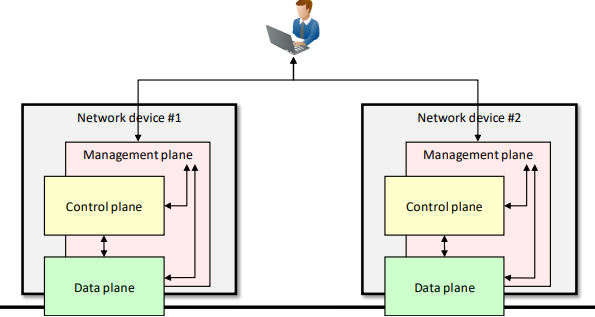
\includegraphics[width=0.90\textwidth]{figure/control_data_plane.png}
    %\caption{qemu-system-arm-version} 
\end{figure}


\subsection{Goal of SND: break the verticality}
how: physical separation between the data plane and the control plane $\rightarrow$ some devices with only the data plane and some devices with only the control plane 

\begin{figure}[h]
    \centering
    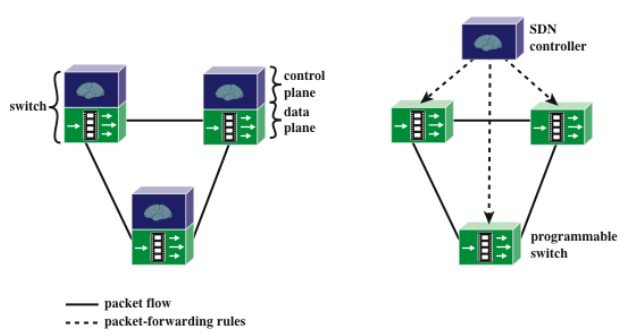
\includegraphics[width=0.90\textwidth]{figure/SDN_config.png}
    %\caption{qemu-system-arm-version} 
\end{figure}

\subsection{SDN switches}
\begin{itemize}
    \item SDN switches are simple $\rightarrow$ they execute always the same low level application (read and apply the routing table), quite fast, cheaper.
    \item SDN controller $\rightarrow$ it has all the intelligence
\end{itemize}

\subsection{3 pillars of SDN}
\subsubsection{Separate control plane and data plane}
  \begin{itemize}
    \item Every SDN switches have their own routing table written by the SDN controller (which embeds the control plane)
    \item SDN controller as an application to which you may add new features by integrating new program
    \item Application and switches has a standard interface to talk each other. (called southbound $\rightarrow$ it permits to make a communication between a lower level network and higher lever network)
    \item Advantages
      \begin{itemize}
        \item Easy to change routing logic
        \item Switches became simpler, faster, cheaper and easy to replace a vendor with another 
      \end{itemize}
  \end{itemize}

\subsubsection{Simple data plane (“plumbing”)}
  \begin{itemize}
    \item Perform “forward to” or “drop”
    \item A way to create “network pipes” (hence plumbing)
    \item The couple match $\rightarrow$ action can be used to create bridge (matching MAC addresses), a router (longest prefix match)
  \end{itemize}

\subsubsection{Centralization of the control plane}
  \begin{itemize}
    \item Software has a view of the ENTIRE network $\rightarrow$ easy to manage
    \item Can even export a “big switch” abstraction
      \begin{itemize}
        \item Big switch abstraction hides internal details of the networks, if I use it I can see only the info about which port is used for the input and for the output
        \item Allow the software to set high level commands
          \begin{itemize}
            \item Set a given configuration to all the edge ports 
            \item Create a direct path from port A to port B
          \end{itemize}
        \item The software can use the normal view (with the visibility of the internals of the net) or “big switch” view
      \end{itemize}
  \end{itemize}

Different implementation of centralized control
\begin{figure}[h]
    \centering
    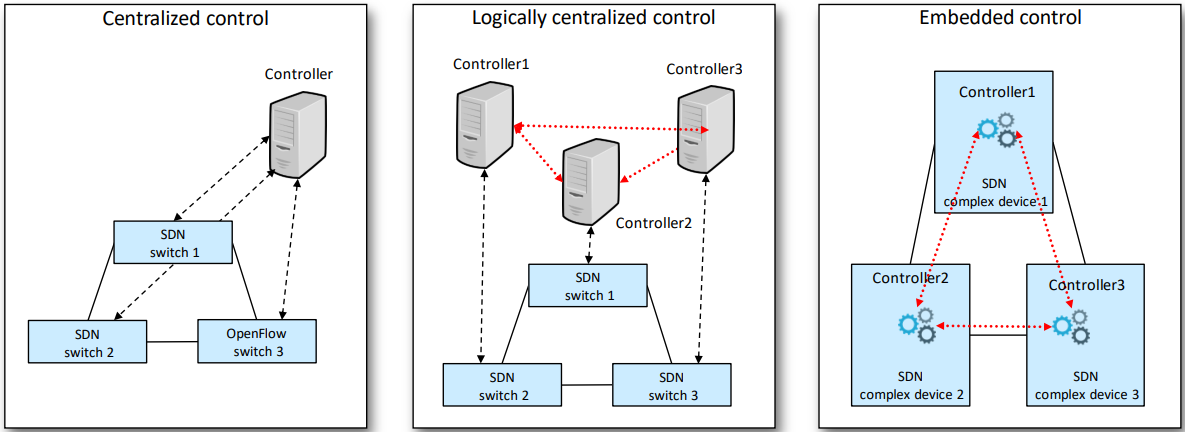
\includegraphics[width=0.90\textwidth]{figure/different_centralized_control.png}
    %\caption{qemu-system-arm-version} 
\end{figure}
  \begin{itemize}
    \item The second there are the problem about the change of the routing table and the consistency of it
    \item The third one is still acceptable because the only difference between it and the normal way is that you may change the logic from ethernet switch to IP routers
  \end{itemize}

Centralized vs logically centralized control
  \begin{itemize}
    \item The SDN is an approach to architecting the network control plane, where the behavior of the net is to determine by software which is logically separated from the network device
      \begin{itemize}
        \item The software could run in the network devices, a set/cluster of dedicated/shared servers or any combination of those
        \item So we are not mandated to use physically centralized controller and a logic one is possible
        \item We can even imagine a complex device that includes both data and control plane
      \end{itemize}
  \end{itemize}

Logically centralized control
  \begin{itemize}
    \item Advantages
      \begin{itemize}
        \item More robust (if there is any fault on one SDN controller another one can replace the faulty one)
        \item Faster decision (some decisions can be taken locally)
        \item More scalability (no big amount of info to only one centralized controller)
      \end{itemize}
    \item Problems
      \begin{itemize}
        \item Complex
        \item Theoretical limit because a distributed data store cannot simultaneously provide more than two of these things: Consistency, Availability, Partition tolerance (CAP theorem)
        \item This implementation guarantees Eventual Consistency
          \begin{itemize}
            \item After an object is updated, it may happen that if I access the same object from a different node I will have a different value. So I need a little period of time that after that I will have always consistency
            \item Impact to the top level application $\rightarrow$ the SDN controller has to provide primitives to synchronize data among the different running instances
            \item Programmers don’t want to write distributed applications (SDN controller should provide a development model in which programmers think about creating “monolithic” applications, SDN controller should automatically and transparently execute multiple instances of the above app, and the data synchronization among different instances should be performed automatically)
            \item This may lead to performance issues so SDN controllers export primitives that facilitate the implementation of distributed applications and developers must be aware that their apps can be executed in multiple instances
            \item Synchronization primitives may not be part of the southbound interface
          \end{itemize}
      \end{itemize}
  \end{itemize}

\subsubsection{Context-based forwarding}
  \begin{itemize}
    \item Not originally present in SDN
    \item The control path can take decisions at run-time, based on the actual traffic
    \item The switch can send a packet to the controller where the control application will determine how to handle that traffic
  \end{itemize}

\subsection{OPENFLOW}
\begin{figure}[h]
    \centering
    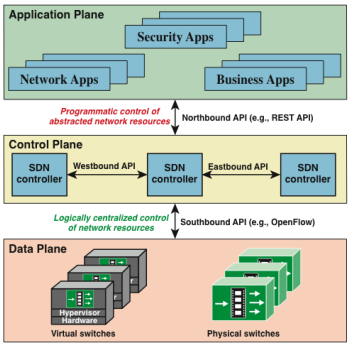
\includegraphics[width=0.90\textwidth]{figure/SDN_architecture.png}
    %\caption{qemu-system-arm-version} 
\end{figure}
\begin{itemize}
    \item OpenFlow is a protocol
    \item in a nutshell
    \begin{itemize}
        \item sends forwarding rules to the switch
        \item Receives from the switch the packets that may not match any rules
        \item Can inject packets in the switch
        \item Asks for switch statistic and gets data backs
    \end{itemize}
\end{itemize}
\subsubsection{Architecture}
\begin{itemize}
    \item Data plane
    \begin{figure}[h]
    \centering
    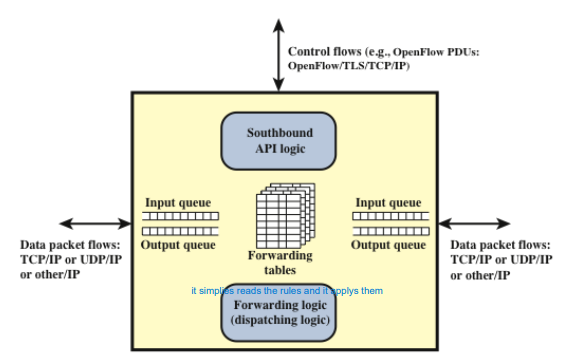
\includegraphics[width=0.90\textwidth]{figure/data_plane.png}
    %\caption{qemu-system-arm-version} 
\end{figure}
    \begin{itemize}
        \item main component: OpenFlow switch
        \begin{figure}[h]
            \centering
            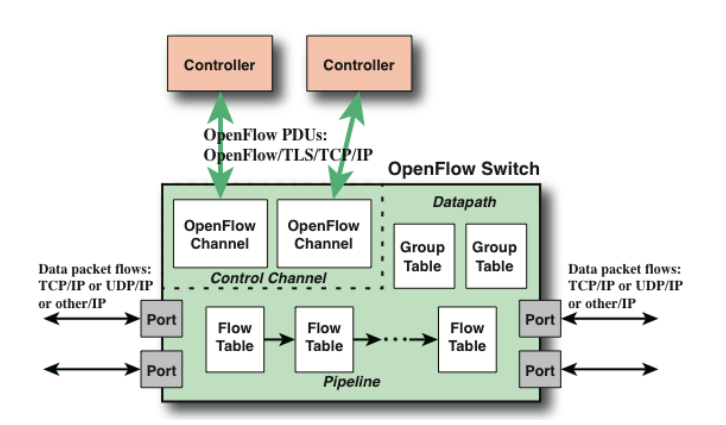
\includegraphics[width=0.90\textwidth]{figure/OpenFLow_switch.png}
            %\caption{qemu-system-arm-version} 
        \end{figure}
        \item Action: 
        \begin{itemize}
            \item Forwarding table has a hierarchy
            \item Forwarding logic read the rules and apply them
            \item Southbound API logic communicate with the SDN controller
        \end{itemize}
        \item Context-based control plane (optional)
        \begin{itemize}
            \item The control place can take decision at run-time, based on the actual traffic
            \begin{itemize}
                \item in IP, decision are taken based on the net topology
            \end{itemize}
            \item The switch can send a packet to the controller when some more intelligence is needed to handle that traffic
            \item Context-based control path
            \begin{itemize}
                \item Switch sends a packet to the controller, it examines the packet and may send it back with the proper forwarding decision, and may add new forwarding rules in the switch
                \item Controller can customize the forwarding rules based on the traffic itself
                \item Can implement directly part of the data plane
                \item Switch may act ad a \textbf{cache} for the forwarding decision
            \end{itemize}
            \item We can have reactive and proactive configuration of OpenFLow entries
            \begin{figure}[h]
                \centering
                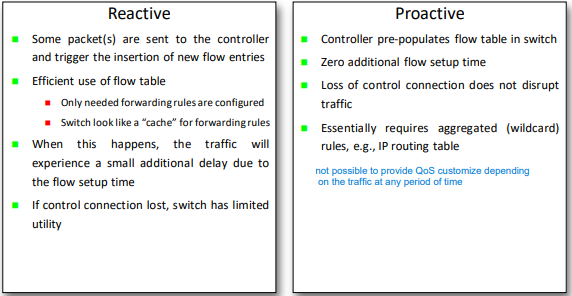
\includegraphics[width=0.90\textwidth]{figure/reactive_proactive.png}
                %\caption{qemu-system-arm-version} 
            \end{figure}
            \item We can have fine-grained or aggregates routing
            \begin{figure}[h]
                \centering
                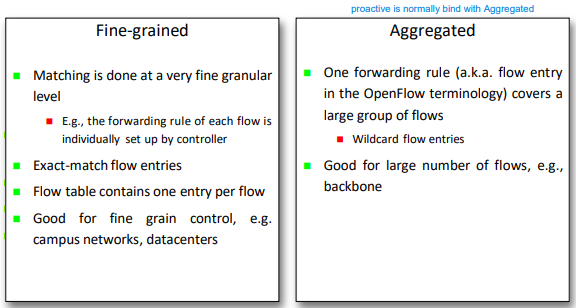
\includegraphics[width=0.90\textwidth]{figure/FineGrained_aggregated.png}
                %\caption{qemu-system-arm-version} 
            \end{figure}
            \begin{itemize}
                \item If we choose proactive configuration, we have to use aggregated routing
                \item If we choose reactive configuration, we are freely to use all
            \end{itemize}
            \item Flow Table Entry
            \begin{itemize}
            \begin{figure}[h]
                \centering
                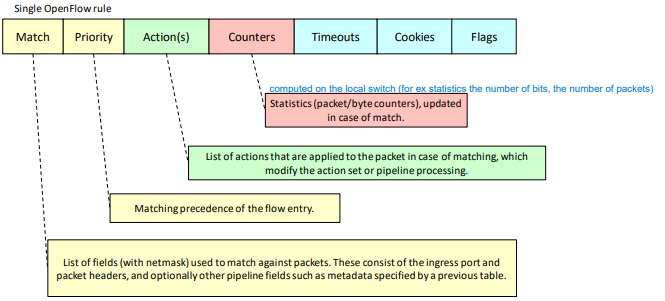
\includegraphics[width=0.90\textwidth]{figure/Flow_table.png}
                %\caption{qemu-system-arm-version} 
            \end{figure}
                \item Flow rule is a traffic flow abstraction
                \begin{enumerate}
                    \item Uses OpenFlow fields
                    \item Can connect 3 OpenFlow switch
                    \item May cross multiple OpenFlow switches
                    \item Is isolated from other FlowRules
                    \item can be a flow table entry in a single switch
                \end{enumerate}
                \item Flowmod is a OpenFLow message used to instantiate, modify, delete a flow rule on a single switch
                \item Match
                \begin{enumerate}
                    \item Arbitrary bits in header
                    \item Allow any flow granularity
                    \item L7 fields not currently supported
                    \item It has lot of types of filtering based on protocols L2-L4
                    \item Wildcard supported
                \end{enumerate}
                \item Priority
                \begin{enumerate}
                    \item The matching process start with the flowrules at the highest priority
                    \item 16 bit value
                \end{enumerate}
                \item Counters
                \begin{enumerate}
                    \item Statistic computed on the local switch and propagated through OpenFlow to the SDN controller
                \end{enumerate}
                \item Common action
                \begin{enumerate}
                    \item Forward
                    \item Drop
                    \item Overwrite header field
                    \item Push or pop field
                    \item Forward at specific bitrate
                    \item Multiple actions can be supported in the same match
                \end{enumerate}
            \end{itemize}
        \end{itemize}
        \item SDN controller
        \begin{itemize}
            \item Architecure
            \begin{itemize}
                \item Southbound interface for the communication of dataplane (with different protocol communiate directly with switches)
                \item Service Abstraction Layer (may create that big switch abstraction when it is needed $\rightarrow$ virtual logical rappresentation for the top layer)
                \item Core network services
                \item Northbound interface for the application plane
                \item Additional services
            \end{itemize}
            \item Complex software that allow the control of the entire network infrastructure
            \item Enable programmability of the network (OpenFLow controllers)
            \item Support heterogeneous network domains
            \item Business consideration $\rightarrow$ guardare le slides perchè non sò quanto effettivamente siano utili
        \end{itemize}
    \end{itemize}
\end{itemize}
\subsubsection{SFCs (applications of SDN to Service Function Chain) }
\begin{itemize}
    \item \textbf{DEF:} Different dedicated hardware appliances to provide added-value services
    \begin{figure}[h]
        \centering
        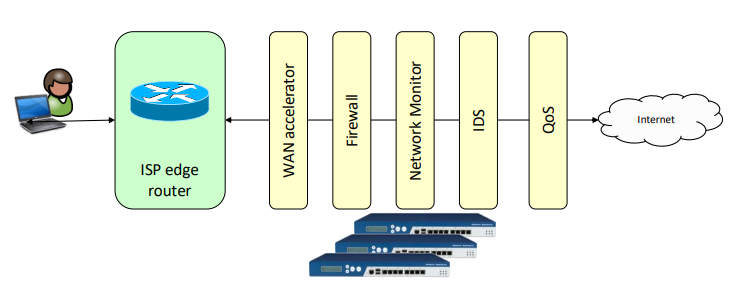
\includegraphics[width=0.90\textwidth]{figure/service_function_chain.png}
        %\caption{qemu-system-arm-version} 
    \end{figure}
    \item Problems of SFC:
    \begin{itemize}
        \item hardware resources are not used at best
        \begin{itemize}
            \item For ex. the firewall can analize more packet than WAN accelerator can give to its
            \item Service disruption when modifying the service chain
            \item it isn’t easy to differentiate services among tenants (user of the same ISP edge router = inquilini)
        \end{itemize}
    \end{itemize}
    \item SFC with SDN
    \begin{figure}[h]
        \centering
        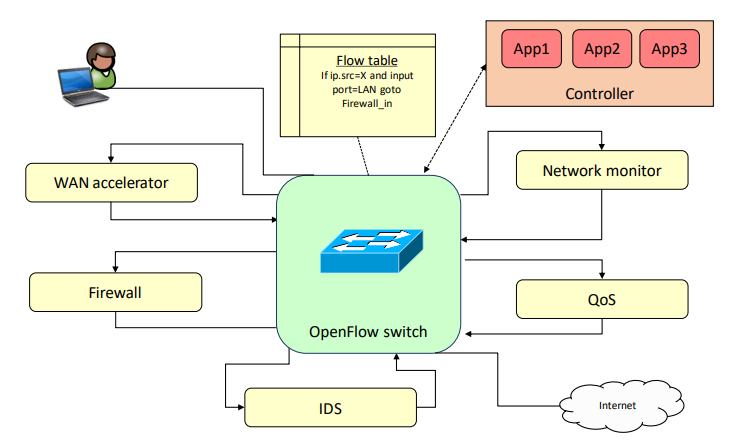
\includegraphics[width=0.90\textwidth]{figure/SFC_with_SDN.png}
    %\caption{qemu-system-arm-version} 
    \end{figure}
    \begin{itemize}
        \item An OpenFlow switch can be installed to connect all boxes together
        \item OpenFlow rules can be used to split the traffic from each user to the proper set of services and rules can be provisioned on demand or pre-previsioned
        \item The controller can be installed locally to the machines
        \item Agility is provisioning new services
        \item Maintenance and reliability
        \item Different customers can have different service chains
        \item Still difficult to partition a physical appliance among different tenants $\rightarrow$ routing done via software
        \item Middleboxes are still hardware-based $\rightarrow$ design, implementation and installation require time
    \end{itemize}
\end{itemize}


\section{Threats}
NIST: circumstances and events that have a negative impact on business operations (destruction, disclosure, modification of info) also the possibility of using a vulnerability to attack
RFC4949: 
  \begin{itemize}
    \item different definitions: 
      \begin{itemize}
        \item a potential for violation of security
        \item any circumstance that can affect a system through unauthorized access
        \item The technical ability of a hostile entity to detect, destroy a friendly system.
        \item An indicator of imminent unwanted events.
      \end{itemize}
    \item 2 possible threats
      \begin{itemize}
        \item Intentional threat: an attack by an intelligent entity
        \item Accidental threat: human errors
      \end{itemize}
  \end{itemize}

\subsection{Different threats}
\begin{itemize}
  \item Eavesdropping: sniffing during net transmission
  \item Fraud: during some transition/communication there are some data/info that are altered in order to obtain extra info
  \item Theft: stealing data and secrets in order to cause harm
  \item Sabotage: create some issue to the system that it will not work in a proper way (DoS)
  \item External attack: the attack is performed outside the organization
  \item Internal attack
\end{itemize}

\section{Vulnerability}
Def: weaknesses that can be exploited by one or more threats

\subsection{Attacks}
ISO 27000: attempt that destroys, exposes, or gains unauthorized access to an asset or unauthorized use of it
IETF RFC 4949: the difference between before is that it is an intentional act
NIST: any kind of malicious activity that attempts to collect, deny, or manipulate information or to an information system resource

\subsection{Security issue}
Generic term to talk about attacks, threats, and vulnerabilities (we can consider it like a box that inside has 3 different boxes: attacks, threats, and vulnerabilities)

\section{Main Security Principles}
Security by design
  \begin{itemize}
    \item Security is implemented during the configuration of the software, not at the end
    \item The original idea: consider some properties that are needed. We cannot apply them always all together
      \begin{itemize}
        \item Least privilege: provide any entity the minimum privilege and resources for the minimum period to complete tasks $\rightarrow$ reduce opportunity of unauthorized access
        \item Separation of Duties: for the completion of a specific activity or access to sensitive objects is dependent on the satisfaction of a plurality of conditions 
        \item Separation of privilege: before performing an action, several conditions have to be passed
        \item Defense in depth: several levels of defense 
        \item Fail secure vs Fail safe: example of the door that can be opened by a badge, if the energy is interrupted and the door will be opened = fail safe. If the door remains forever closed = fail secure. $\rightarrow$ we have to decide what to choose to apply in these cases  
        \item Complete mediation: every request by an entity to access an object in a computer system must be checked with a valid and effective authorization procedure (ex. In the pentagon all the doors are locked and to open them you have to validate at every door)
        \item Last common mechanism: have the minimum level of security /security mechanism in the entire system
        \item Psychological acceptability: a user must be able to understand the user interface and use it without having to interpret complex instructions for the cloud access control mechanism
        \item Weakest link: we have to review the chain of security to detect and resolve the weakest part of the chain
        \item Zero trust: all elements of the system should be considered untrusted so we have to protect individually the elements of my network
      \end{itemize}
  \end{itemize}

\section{Firewall}
\subsection{Definition}
\begin{itemize}
\item NIST:
  \begin{itemize}
    \item a part of the computer system or a network, that is not only one component, that is designed to block unauthorized access
    \item an inter-network connection device that restricts data communication traffic between 2 connected networks
    \item it can be an application installed on a general-purpose computer or a dedicated platform which drops or accepts packets on a network
    \item usually sets on zone borders
    \item it has rules restricting which ports are open
  \end{itemize}
\item RFC 4949: 
  \begin{itemize}
    \item a device or program that controls the flow of network traffic
    \item FIREWALLING $\rightarrow$ FIREWALL IS NOT ALWAYS A SINGLE COMPUTER 
      \begin{itemize}
        \item Maybe 2 different computers can have the same firewall1 but maybe they have another different firewall2 each
        \item Def: 
          \begin{itemize}
            \item Rfc4949: different types of firewall are used like external router that blocks attacks that use IP to break security and proxy servers that block attacks in a higher-layer protocol
            \item The internal router prevents traffic from leaving the protected network except through the proxy servers
          \end{itemize}
      \end{itemize}
  
    
    \item 2 main problems
    \begin{itemize}
        \item Which traffic is good or not
        \item Interaction between other network administrators of my company
    \end{itemize}
    
    \item Characteristics
    \begin{itemize}
        \item The aim is to prevent an attacker from compromising an host with malicious traffic
        \item Inserted between the premises networks and the internet to establish a controlled link and have a sort of security wall
        \item Aim of the perimeter is to protect the premises network from internet-based attacks and to provide a single choke point where security can be imposed
        \item Can be set also internal firewall to segregate portions of an internal network and control internal traffic
    \end{itemize}
    \item Difficult to set the criteria by which packets are denied
    \end{itemize}
\end{itemize}

Nowadays is not possible to have only 1 firewall between the LAN and the internet because in some case also the communication between 2 hosts in the same LAN can be done passing from the host1 to internet and from the internet to the host2.

\subsection{Piccola digressione}
Struttura pacchetto:
H = Header

| H2 | H3 | H4 | H7 | Payload |

| eth | ip | tcp | http | Payload |




\subsection{Main design goals}
\begin{itemize}
  \item In my zone, I have several connections to the net and it is important to have a firewall on each connection
  \item Only authorized traffic (as defined by the local security policy) will be allowed to pass
    \begin{itemize}
      \item Policy determines:
        \begin{itemize}
          \item Access control over and only traffic, it cannot do authentication of the user (if I lock a specific IP/MAC address I block only the traffic flow from that device but if the bad guy uses another IP/MAC address, he can send packets)
          \item Accept or deny
          \item Must be immune to penetration itself $\rightarrow$ our firewall is developed taking into account to define a secure solution $\rightarrow$ so it is trusted
        \end{itemize}
    \end{itemize}
  \item What can do?
    \begin{itemize}
      \item Keep unauthorized users out of the protected network
      \item Prohibits vulnerable services from entering or leaving the network
      \item Protect from IP spoofing and routing attacks
      \item Provides a location for monitoring security-related events (it registers and analyzes the activities that can be malicious for the networks)
      \item Convenient platform for several internet functions that aren’t secure
      \item Control traffic between “zones of trust” (inside our network for example we can have different zones with different levels of trust)
      \item Can be the platform for implementing VPN 
    \end{itemize}
  \item Type of control that can be done
    \begin{itemize}
      \item Service/application control
        \begin{itemize}
          \item Which types of internet services can be accessed inbound or outbound
        \end{itemize}
      \item Direction control
    \end{itemize}
  \item Type of control that cannot be done
    \begin{itemize}
      \item Protect against internal threats
      \item Protect against connection that bypass it
      \item Protect against completely new threats
      \item Protect against viruses and worms
      \item Set itself up correctly (it is not plug and play)
    \end{itemize}
  \item Problems 
    \begin{itemize}
      \item Interfere with the internet end to end communication model
      \item False sense of perfect security
      \item Increase inconveniences for users
    \end{itemize}
\end{itemize}

\subsection{Firewall Configuration}
The position of a FW is based on what policy it implements and the configuration depends on how the FW handle network traffic:
  \begin{itemize}
        \item Definition: set of rules, default action applied and resolution strategy based on:
          \begin{itemize}
            \item IP addresses
            \item Address ranges
            \item Protocol
            \item Applications
            \item Content types
          \end{itemize}
        \item Composition: \(r = (C, a)\) 
          \begin{itemize}
            \item (C) Conditions: single or a range of values that represent the possible values of the corresponding field in actual packets which match the rules
            \item (a) actions: allowed $\rightarrow$ forward packets; deny $\rightarrow$ discard packets
            \item So, the packets are allowed or denied by a specific rule if the header matches all the conditions of these rules
          \end{itemize}
        \item Default action
          \begin{itemize}
            \item Applied if the packet doesn’t meet all the conditions of any rule
            \item Problem: if more than one rule matches the traffic we need to define a resolution strategy
          \end{itemize}
        \item Resolution strategy
          \begin{itemize}
            \item More than one rule matches the packets
            \item Example: first matching rule (FMR), last matching rule (LMR), allow takes precedence (ATP) $\rightarrow$ allow rule is respected instead of the deny rule, Deny Takes Precedence (DTP), Most Specific Takes Precedence (MSTP), Least Specific Takes Precedence (LSTP)
          \end{itemize}
        \item Denylist/blacklist
          \begin{itemize}
            \item All that is not explicitly forbidden is permitted (the rules deny the traffic that match the rules, and the default rules are to allow all traffic that don’t match any rules)
            \item Lower security 
            \item Easier to manage
          \end{itemize}
        \item Allowlist/whitelist
          \begin{itemize}
            \item All that is not explicitly permitted is forbidden (default action = deny)
            \item Higher security
            \item More difficult to manage
          \end{itemize}
        \item General access control list
          \begin{itemize}
            \item Rules can be allowed or denied
            \item Default action can be allowed or denied
            \item Each rule has a specific priority order
            \item Most used
            \item It is common to make anomalies among rules
          \end{itemize}
      \end{itemize}
    Different types of FW based on:
      \begin{itemize}
        \item Filtering $\rightarrow$ which type of the header/payload is able to filter
        \begin{figure}[h]
            \centering
            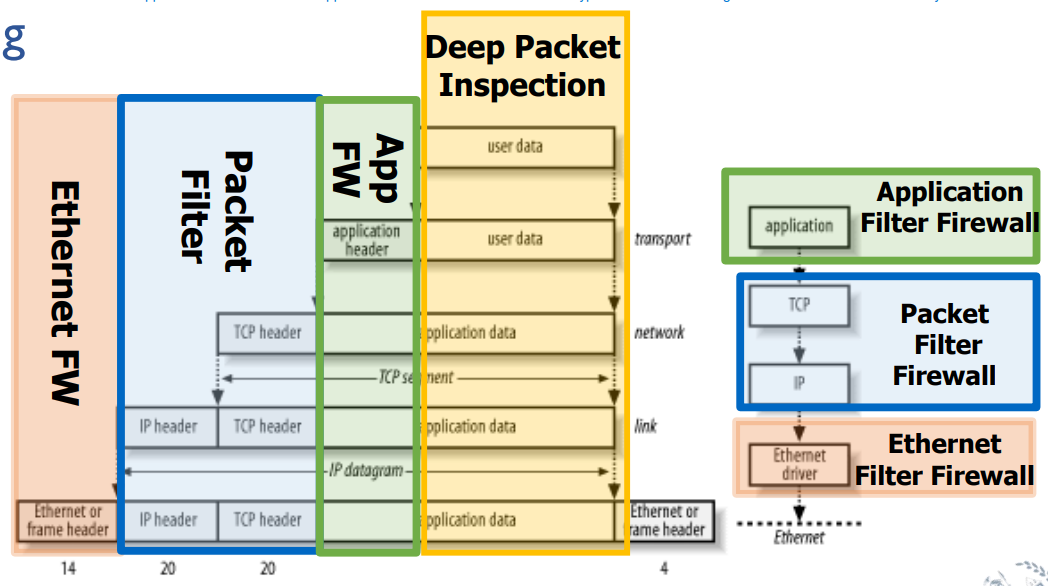
\includegraphics[width=0.90\textwidth]{figure/filtering.png}
             %\caption{qemu-system-arm-version} 
        \end{figure}
        \item State
        \item Proxy
        \item Other $\rightarrow$ enc/dec specific network (for VPN), network address translation, unified threat management
      \end{itemize}

\subsection{Types of FW}
The types of FW differs by each other in 4 different categories: which type of the header/payload is able to filter, state, proxy and other (enc/dec specific network that are used in VPN, network address translation, unified threat management)
\begin{itemize}
  \item Packet filter (most common) 
    \begin{itemize}
      \item Rules based on info in the IP packet header at layer 3 and 4
        \begin{itemize}
          \item IP source
          \item IP destination
          \item Protocol (at layer 4)
          \item Source port
          \item Destination port
        \end{itemize}
      \item Advantages
        \begin{itemize}
          \item Simple way to work
          \item Very fast (layers that are inspected are low)
          \item Good scalability
          \item Low cost
          \item Typically transparent to user
        \end{itemize}
      \item Disadvantages
        \begin{itemize}
          \item Vulnerable to attacks 
          \item Improper configuration cause security breaches
          \item Complex to configure
          \item Don’t support advanced user authentication schemes
          \item Cannot prevent attacks that employ application-specific vulnerabilities or functions
          \item Logging functionality is limited
        \end{itemize}
      \item Attacks
        \begin{itemize}
          \item IP spoofing $\rightarrow$ countermeasures: discard packets with an inside source address but it is coming from an external interface
          \item Source routing attack (source station specifies the route that a packet should take as it crosses the internet) $\rightarrow$ countermeasures: discard all packets that use this option
          \item Tiny fragment attack (the attacker uses the IP fragmentation option to create extremely small fragments and force the TCP header info into a separate packet fragment producing issues at layer 4) $\rightarrow$ countermeasures: enforce a rule that the first fragment of a packet must contain a predefined minimum amount of the transport header. If the first fragment is rejected, the filter can remember the packet and discard all subsequent fragments
        \end{itemize}
      \item Example
        \begin{figure}[h]
            \centering
            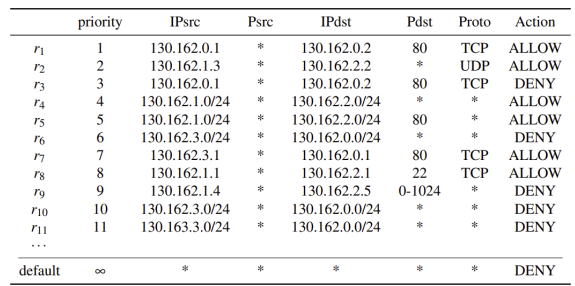
\includegraphics[width=0.90\textwidth]{figure/filter_table.png}
            %\caption{qemu-system-arm-version} 
        \end{figure}
    \end{itemize}
  \item Ethernet firewall
    \begin{itemize}
      \item Definition: it is used to set up and maintain the table of rules that inspect ethernet frames
      \item Similar to a packet filter but simpler because the ethernet protocol is much simpler than the IP protocol
      \begin{figure}[h]
        \centering
        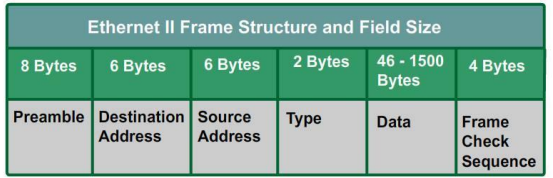
\includegraphics[width=0.90\textwidth]{figure/eth_firewall.png}
        %\caption{qemu-system-arm-version} 
      \end{figure}
      \item Rules
        \begin{itemize}
          \item MAC address filtering $\rightarrow$ filter traffic based on the MAC address of the sender or receiver (helpful for ensuring specific devices have or don’t have network access)
          \item Virtual LAN tagging $\rightarrow$ allow or block specific VLANs, providing control over which frames are allowed to pass through certain ports
          \item Some of them can filter based on ARP fields
        \end{itemize}
    \end{itemize}
  \item Application firewall (layer 7) 
    \begin{itemize}
      \item Definition: firewall that controls input/output or system calls of an application or service 
        \begin{itemize}
          \item it can block an email that contains a type of attachment that is not permitted
          \item it can block connections over which specific actions are being performed (ex: FTP command (put), which allows users to write files to the FTP server)
          \item allow or deny web pages that contain particular types of active content that has a compromised or revoked CA
        \end{itemize}
      \item WEB APPLICATION FIREWALL (most used)
        \begin{itemize}
          \item Definition: application firewall that monitors filters and blocks HTTP traffic as it travels to and from website or web application (ex of attacks that prevent: Cross Site Scripting and SQL injection)
        \end{itemize}
        \begin{figure}[h]
            \centering
            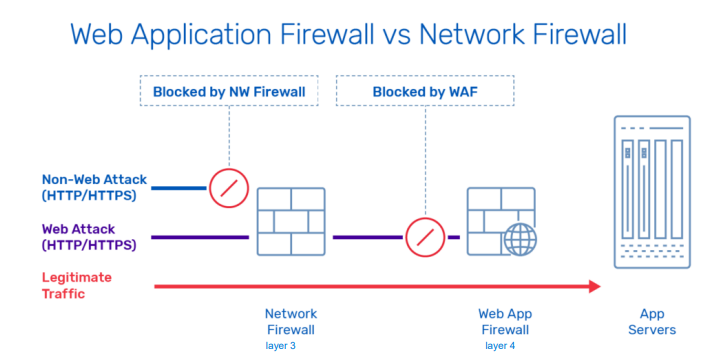
\includegraphics[width=0.90\textwidth]{figure/web_appl_firewall.png}
            %\caption{qemu-system-arm-version} 
       \end{figure}
    \end{itemize}
  \item Proxy
    \begin{itemize}
      \item Definition: it is a server application that broke the communication between server and client $\rightarrow$ client asks for a resource from a proxy server, which evaluates the request and performs the required network transaction thanks to the real server that provides to it the resources
      \item Breaks client-server model
        \begin{itemize}
          \item More protection for the server
          \item May authenticate the client
          \item Not transparent to the client
        \end{itemize}
        \begin{figure}[h]
            \centering
            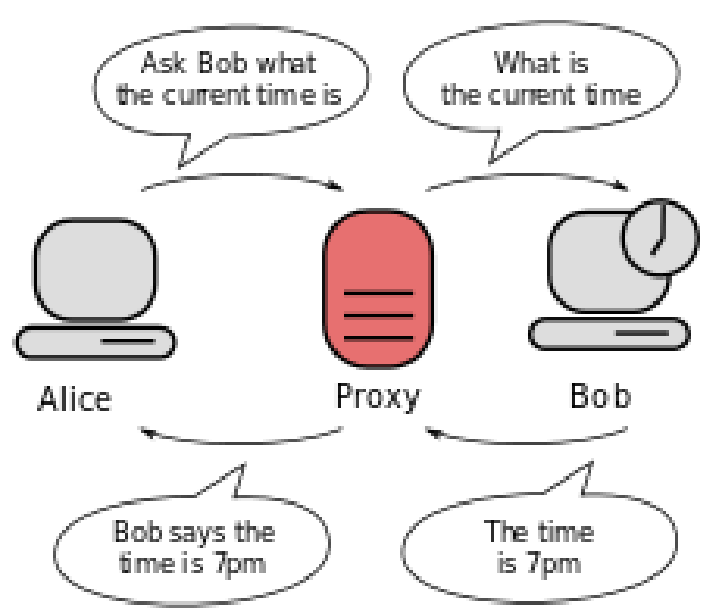
\includegraphics[width=0.90\textwidth]{figure/proxy.png}
            %\caption{qemu-system-arm-version} 
        \end{figure}
      \item It is also similar to a cache
      \item Types
        \begin{itemize}
          \item Open proxies $\rightarrow$ in the middle between internet and internet
          \item Reverse proxy 
            \begin{itemize}
              \item Proxy in the middle between the internet and the internal web server that it has to protect
              \item Encryption/SSL acceleration
              \item Load balancing
              \item Caching
              \item Security (isolation)
            \end{itemize}
        \end{itemize}
      \item Other types
        \begin{itemize}
          \item Application level gateway
            \begin{itemize}
              \item Source contacts the gateway using TCP/IP application and the gateway asks the user for the name of the remote host to be accessed
              \item When the source responds and provides valid user ID and auth info, the gateway contacts the application on the remote host and gives TCP segments containing the application data between the two endpoints
              \item If the gateway doesn’t implement proxy code for a specific application, the service is not supported and cannot be forwarded across the firewall
              \item The gateway can be configured to support only specific features of an application that the network administrator considers acceptable while denying all other features
              \item Advantage
                \begin{enumerate}
                  \item More secure than a Packet Filter
                  \item Easy to log and audit all incoming traffic at the application level
                  \item Is not needed to audit and verify TCP and IP level
                  \item Can perform user-level authentication
                  \item Can do intelligent filtering
                  \item Can be combined with caching
                  \item Can do good logging
                \end{enumerate}
              \item Disadvantages
                \begin{enumerate}
                  \item Additional processing overhead on each connection
                  \item There are 2 connections between the end user and the gateway in the middle that examine and forward the traffic
                  \item Require different servers for each service
                    \begin{enumerate}
                      \item Delay in supporting new applications
                      \item Heavy on resources
                      \item Require modifications to clients
                    \end{enumerate}
                \end{enumerate}
            \end{itemize}
          \item Circuit level gateway
            \begin{itemize}
              \item Also referred to as a transparent proxy firewall
              \item Breaks TCP/UDP connection
                \begin{enumerate}
                  \item Protect against TCP handshake attack
                  \item Protect against IP fragmentation
                \end{enumerate}
            \end{itemize}
          \item Stateful firewall
            \begin{itemize}
              \item Def STATE: packet filter doesn’t take into consideration any higher-layer context and most standardized applications that run on top of TCP follow a client/server model
              \item When a packet arrives, whether it is an egress or ingress packet, the stateful filtering firewall checks whether the packet belongs to an existing connection against its state table. If the packet doesn’t match any rule, the firewall controls the table related to the stateless rules.
              
              \begin{figure}[h]
                \centering
                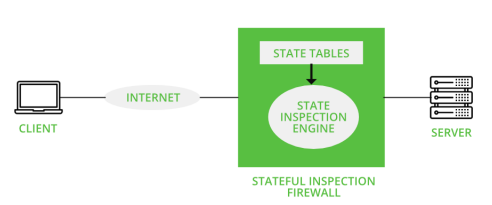
\includegraphics[width=0.90\textwidth]{figure/statefull_firewall.png}
                %\caption{qemu-system-arm-version} 
              \end{figure}
                \begin{enumerate}
                  \item If the packet matches a rule, the firewall saves the info for later use
                  \item SYN packet $\rightarrow$ creates a new entry in the state table
                  \item If the packet doesn’t belong to an existing connection or it isn’t a SYN packet $\rightarrow$ discarded
                  \item When a network connection ends $\rightarrow$ it is removed from the state table
                \end{enumerate}
              \item State keep track of the connection status and filter based on it
                \begin{enumerate}
                  \item TCP
                    \begin{enumerate}
                      \item is implemented with sequence number
                      \item Only the first packet of the connection
                    \end{enumerate}
                  \item UDP 
                    \begin{enumerate}
                      \item is implemented just with the tuple source address, source port, destination address, and destination port.
                      \item All the other packets of the connection
                    \end{enumerate}
                \end{enumerate}
              \item Stateful filtering keeps track of connections between an internal host and an external host
              \item Connection state indicates whether it is a TCP connection or a UDP connection and whether the connection is established
              \item Connection states are stored in a state table
            \end{itemize}
        \end{itemize}
    \end{itemize}
\end{itemize}
            
\subsection{Firewall solutions}
\begin{itemize}
  \item Open source
    \begin{itemize}
      \item Freely available
      \item Have gained wider acceptance as are built
      \item Incorporate fewer features
    \end{itemize}
  \item Proprietary
    \begin{itemize}
      \item Owned by an entity that has an exclusive right to them
    \end{itemize}
  \item Hardware
    \begin{itemize}
      \item Are specialized separate devices that inspect traffic
      \item It has a software firewall inside
    \end{itemize}
  \item Software
    \begin{itemize}
      \item Runs as a program or service on a device
      \item Disadvantages $\rightarrow$ a malware infection on the device on which it is running could also compromise the software firewall
    \end{itemize}
  \item Host
    \begin{itemize}
      \item Software firewall that runs on (and protects) a single endpoint device
      \item All modern OSs include a host-based firewall
      \item Topology independent in fact all attacks must go through the firewall
      \item Extensible without the need of altering the network configuration
      \item Application-centric in fact a user can create an opening in the firewall for each specific application $\rightarrow$ this approach is more secure than permanently opening a port in the firewall.
    \end{itemize}
  \item Appliance
    \begin{itemize}
      \item It is a separate hardware device designed to protect an entire network
    \end{itemize}
  \item Virtual
    \begin{itemize}
      \item Runs in the cloud
      \item Are designed for settings in which deploying firewalls would be difficult or impossible
    \end{itemize}


\item Position
\begin{itemize}
  \item Screening router
  \begin{figure}[H]
    \centering
    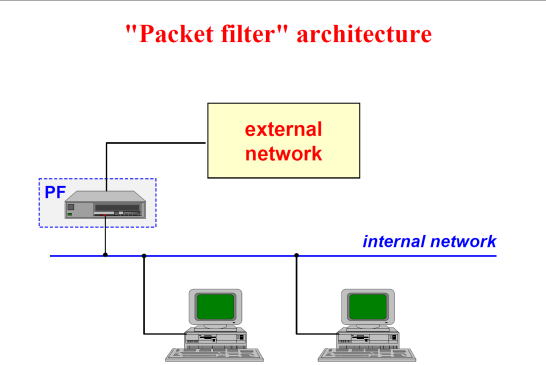
\includegraphics[width=0.90\textwidth]{figure/packet_filter.png}
    %\caption{qemu-system-arm-version}  
  \end{figure}
  \item Dual homed gateway
  \begin{figure}[H]
    \centering
    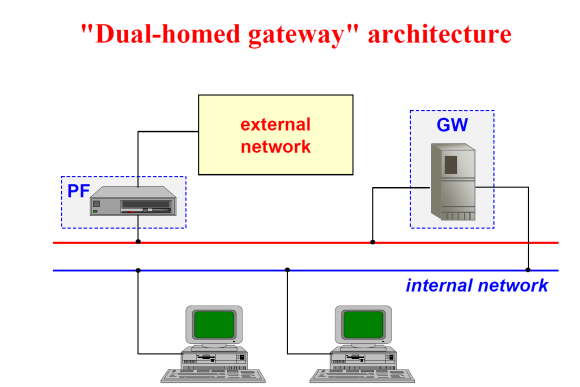
\includegraphics[width=0.90\textwidth]{figure/Dual-home_gateway.png}
    %\caption{qemu-system-arm-version}  
  \end{figure}
  \item Screened host gateway
  \begin{figure}[H]
    \centering
    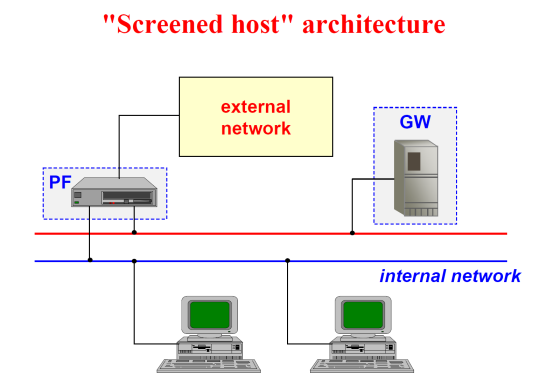
\includegraphics[width=0.90\textwidth]{figure/screened_host.png}
    %\caption{qemu-system-arm-version}  
  \end{figure}
  \item Screened subnet
  \begin{figure}[H]
    \centering
    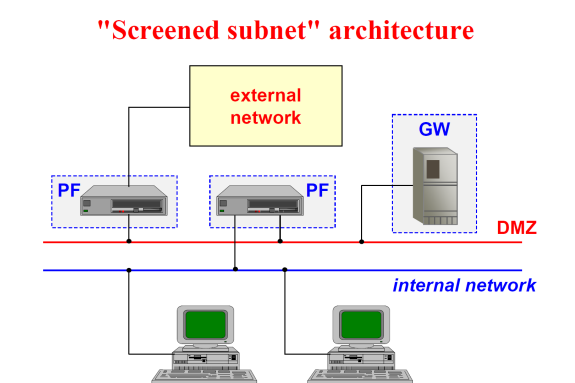
\includegraphics[width=0.90\textwidth]{figure/screened_subnet.png}
    %\caption{qemu-system-arm-version}  
  \end{figure}
  \begin{figure}[H]
    \centering
    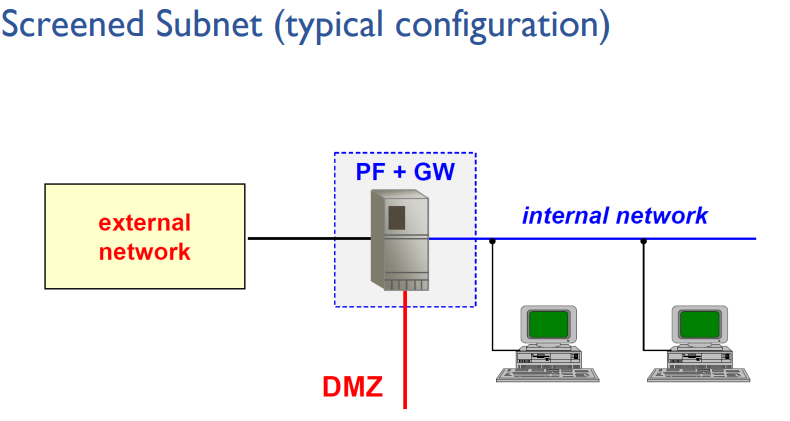
\includegraphics[width=0.90\textwidth]{figure/screened_subnet_2.png}
    %\caption{qemu-system-arm-version}  
  \end{figure}
  \item DMZ
    \begin{itemize}
      \item Definition: Perimeter network segment that is logically between the internal and external networks.
      \item Purpose: enforce the internal network’s information assurance policy for external info exchanged and to provide external, untrusted sources with restricted access to releasable info while shielding the internal net from external attacks
    \end{itemize}
\end{itemize}
\end{itemize}
\subsection{Firewall policy rules anomaly}
\begin{itemize}
  \item Definition: A policy rules anomaly occurs when a set of policies is simultaneously satisfied. This implies that the combined actions of the policy rules may produce different results depending on the order of execution of these actions
  \item Types
    \begin{itemize}
      \item Error
        \begin{itemize}
          \item Occurs when the attempts to enforce the policy actions fail
            \begin{itemize}
              \item Ex: an action is not supported, a type of syntax is not supported
            \end{itemize}
          \item Resolution $\rightarrow$ detect and solve
        \end{itemize}
      \item Conflict
        \begin{itemize}
          \item Occurs when the effect of one security policy is influenced or altered by another one
          \item Resolution $\rightarrow$ policy systems must provide conflict detection and avoidance or resolution mechanisms to prevent the situation
        \end{itemize}
      \item Sub-optimization (resolution)
        \begin{itemize}
          \item Occurs when redundant rules or other more efficient policy implementations are present
          \item Decrease the performance of my firewall
            \begin{figure}[H]
                \centering
                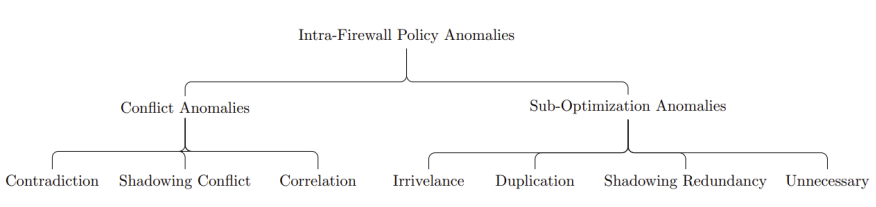
\includegraphics[width=0.90\textwidth]{figure/sub optimization.png}
                %\caption{qemu-system-arm-version}  
            \end{figure}
          \item Anomalies of the sub-optimization:
            \begin{itemize}
              \item Irrelevance
                \begin{enumerate}
                  \item Definition: a policy rule is irrelevant if it doesn’t match any packet that might arrive at the firewall
                  \item Occurs when the source or the destination address of the rules doesn’t match with the subnet protected by the firewall
                  \item Cancellation of an irrelevant policy rule doesn’t alter the policy behavior
                \end{enumerate}
              \item Duplication
                \begin{enumerate}
                  \item Definition: A policy rule \(n_1\) duplicates rule \(n_2\) and vice versa if they specify the same action and match the same packets
                  \item Cancellation of the rule with the lowest priority will not change the policy behavior
                \end{enumerate}
                  \begin{figure}[H]
                    \centering
                    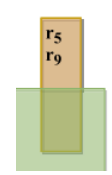
\includegraphics[width=0.15\textwidth]{figure/duplication.png}
                    %\caption{qemu-system-arm-version}  
                \end{figure}
              \item Shadowing redundancy anomaly
                \begin{enumerate}
                  \item A policy rule \(n_1\) is shadowed by the rule \(n_2\)
                  \item \(n_2\) has more priority
                  \item All packets matched by \(n_1\) are also matched by \(n_2\)
                  \item \(n_1\) and \(n_2\) specify the same action
                \end{enumerate}
                  \begin{figure}[H]
                    \centering
                    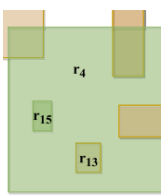
\includegraphics[width=0.15\textwidth]{figure/shadowing_redundancy.png}
                    %\caption{qemu-system-arm-version}  
                  \end{figure}
              \item Shadowing conflict anomaly
                \begin{enumerate}
                  \item As the shadowing redundancy anomaly but \(n_1\) and \(n_2\) specify different actions
                  \item An automatic removal of this anomaly is not possible, the administrator must decide which rule should be removed
                \end{enumerate}
                \begin{figure}[H]
                    \centering
                    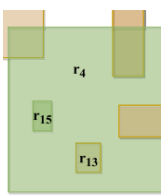
\includegraphics[width=0.15\textwidth]{figure/shadowing_conflict.png}
                    %\caption{qemu-system-arm-version}  
                  \end{figure}
              \item Unnecessary anomaly
                \begin{enumerate}
                  \item A policy rule \(n_1\) is redundant with respect to \(n_2\)
                  \item \(n_1\) and \(n_2\) specify the same action
                  \item \(n_1\) precedes \(n_2\)
                  \item All packets that are matched by \(n_1\) are also matched by \(n_2\)
                \end{enumerate}
                  \begin{figure}[H]
                    \centering
                    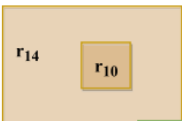
\includegraphics[width=0.15\textwidth]{figure/Unnecessary_anomaly.png}
                    %\caption{qemu-system-arm-version}  
                  \end{figure}
              \item Contradiction anomaly   
                \begin{enumerate}
                  \item \(n_1\) and \(n_2\) are in contradiction if they match the same packets but they specify different actions
                  \item An automatic removal of this anomaly is not possible, the administrator must decide which rule should be removed
                \end{enumerate}
              \item Correlation anomaly
                \begin{enumerate}
                  \item Two policy rules are correlated when they specify different actions and some packets that are matched by \(n_1\) are also matched by \(n_2\) but they are not entirely matched
                  \item An automatic removal of this anomaly is not possible, the administrator must decide which rule should be removed
                \end{enumerate}
                  \begin{figure}[H]
                    \centering
                    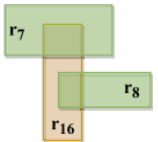
\includegraphics[width=0.15\textwidth]{figure/correlation_anomaly.png}
                    %\caption{qemu-system-arm-version}  
                  \end{figure}
              \item Al-shaer classification
                  \begin{figure}[H]
                    \centering
                    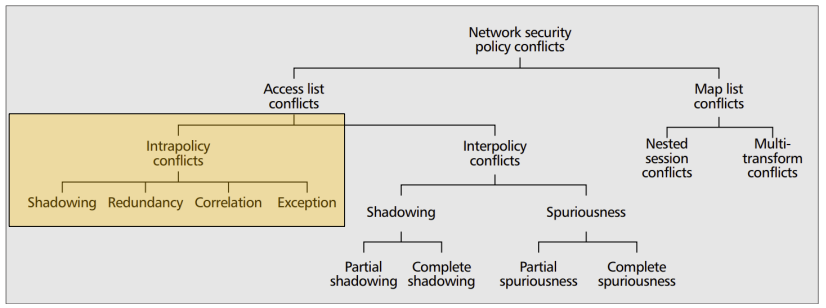
\includegraphics[width=0.90\textwidth]{figure/Al-shaer_classification.png}
                    %\caption{qemu-system-arm-version}  
                  \end{figure}
              \item Valenza classification
                  \begin{figure}[H]
                    \centering
                    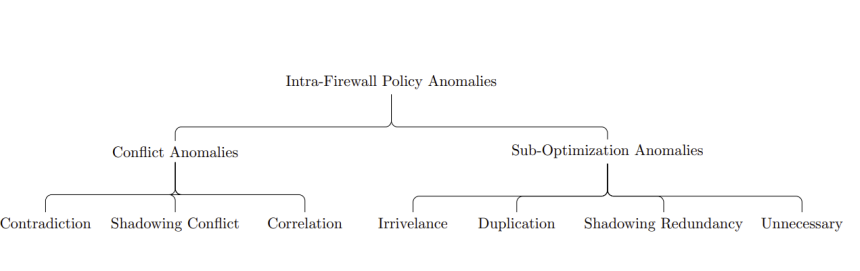
\includegraphics[width=0.90\textwidth]{figure/Valenza_classification.png}
                    %\caption{qemu-system-arm-version}  
                  \end{figure}
            \end{itemize}
        \end{itemize}
    \end{itemize}
\end{itemize}

\section{VPN}
\textbf{DEF:} connectivity realized on a shared infrastructure such that policies (like security, QoS, reliability or addressing) can be enforced as in only one private network. The key elements are the Tunnel (encapsulation of corporate traffic while in transit on the shared network that is not present in some solutions) and the VPN Gateway (that is the termination device on the corporate network and it can be a tunnel endpoint).

\begin{figure}[H]
    \centering
    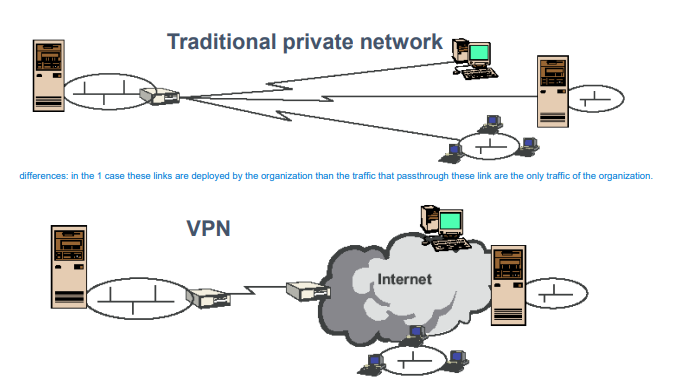
\includegraphics[width=0.90\textwidth]{figure/tradition_vs_VPN.png}
    %\caption{qemu-system-arm-version}  
\end{figure}

\textbf{Why?} it enable cutting costs with respect to expensive cpnnectivity solutions

\subsection{Basic terminology and Scenario}

\begin{itemize}
    \item Flavors
    \begin{itemize}
        \item Access VPN or remote VPN or virtual dial in
        \begin{itemize}
            \item Connects terminal to remote network
            \item Virtualize
        \end{itemize}
        \item Site-to-site VPN
        \begin{itemize}
            \item connect remote networks
            \item virtualizes leased line
        \end{itemize}
        \item End-to-End VPN (the packet is encapsulated in the source and decapsulate in the destination)
        \begin{itemize}
            \item Connect remote hosts
            \item Virtualizes leased line
        \end{itemize} 
        
    \end{itemize}
    \item Deployment scenario
    \begin{itemize}
        \item intranet VPN
        \begin{figure}[H]
            \centering
            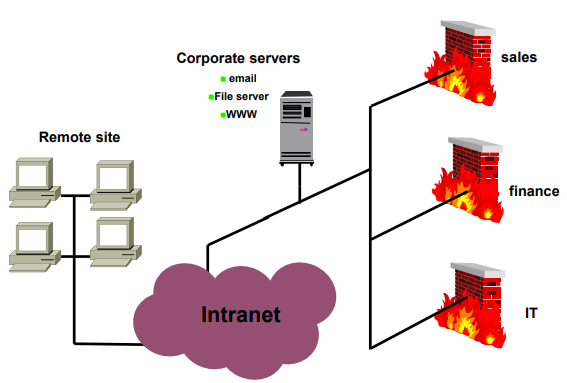
\includegraphics[width=0.90\textwidth]{figure/intranet.png}
            %\caption{qemu-system-arm-version}  
        \end{figure}
        \begin{itemize}
            \item interconnection of the corporate headquarters, remote offices, branch offices, telecommuter, traveling employee (all are related of the same communication)
        \end{itemize}
        
        \item Extranet VPN
        \begin{figure}[H]
            \centering
            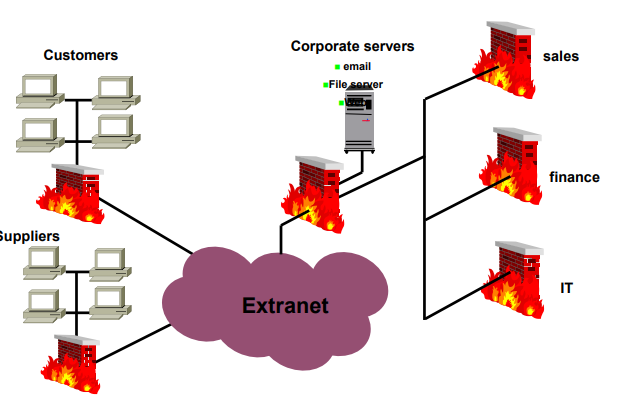
\includegraphics[width=0.90\textwidth]{figure/extranet.png}
            %\caption{qemu-system-arm-version}  
        \end{figure}
        \begin{itemize}
            \item it allows interconnection between 2 different terminal element owned by 2 different company
            \item little more complex to manage because the policy of the 2 terminals can be different and can be not compatible
            \item provide controlled access to an individual customer/partner/provider user
            \item Issues
            \begin{itemize}
                \item restricted access to network resources from interconnected networks by the firewall at the VPN
                \item Overlapping Adreess Spaces by the network address translation
                \item open, standard-based solution that enables interoperability among different organizations
                \item traffic control that avoid partenr traffic compromises performance on corporate network
            \end{itemize}
        \end{itemize}
    \end{itemize}
    \item how to choose the right VPN based on internet access
    \begin{itemize}
        \item centralized
        \begin{itemize}
            \item Remote branches/users use public IP network only to reach headquartes
            \item Internet access only from headquarters
            \item VPN carries also traffic to and from the Internet
            \item Centralized access control and if i want to go on internet i have to pass through the gateway of my company
            \begin{itemize}
                \item Firewall 
            \end{itemize}
            \item Disadvantages
            \begin{itemize}
                \item single point of failure
                \item latency time
                \item the organization must pay internet for the host because it has the power to decide which traffic can go trhough the internet
            \end{itemize}
        \end{itemize}
        \item Distributed (voluntary connection)
        \begin{itemize}
            \item remote branchs/user access the internet throught their IP network connection
            \item VPN is deployed only for corporate traffic
            \item i can decide to open the source communication between the gateway of my company or go directly to the internet
        \end{itemize}
        \begin{figure}[h]
            \centering
            \begin{minipage}[b]{0.45\textwidth}
                \centering
                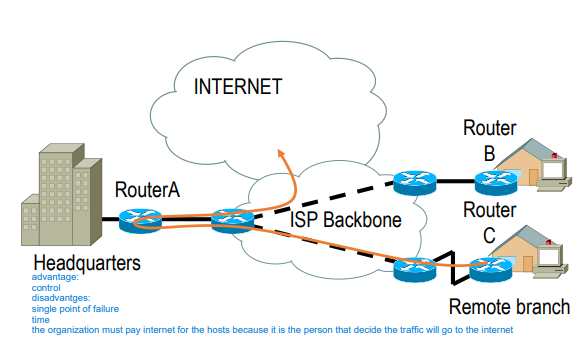
\includegraphics[width=\textwidth]{figure/centralized_VPN.png}
                \caption{centralized}
            \end{minipage}
            \hspace{0.05\textwidth}
            \begin{minipage}[b]{0.45\textwidth}
                \centering
                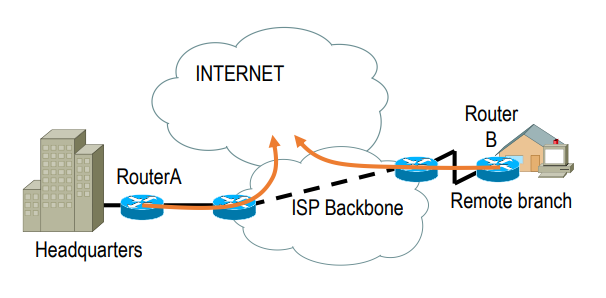
\includegraphics[width=\textwidth]{figure/distributed_VPN.png}
                \caption{distributed}
            \end{minipage}
        \end{figure}
    \end{itemize}
\end{itemize}

\subsection{Deployment Models and Main components}
\begin{itemize}
    \item VPN Features
    \begin{itemize}
        \item Separate data
        \begin{itemize}
            \item Tunneling $\rightarrow$ encapsulate traffic and protect it with a specific policy
        \end{itemize}
        \item increase protection
        \begin{itemize}
            \item Encryption for the confidentiality
        \end{itemize}
        \begin{itemize}
            \item Prevent tampering (manomissione)
            \begin{itemize}
                \item Data ntegrity
            \end{itemize}
            \item identify source
            \begin{itemize}
                \item source Authentication, it doesn't made user auth
            \end{itemize}
        \end{itemize}
    \end{itemize}
    \item s2s VPN tunneling
    \begin{itemize}
        \item Tunnel terminated on gateway
        \begin{figure}[H]
            \centering
            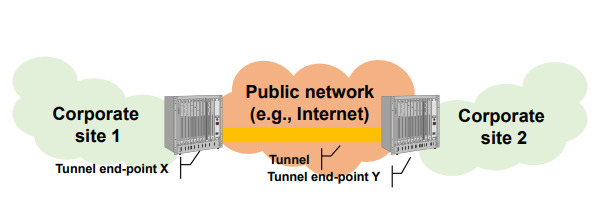
\includegraphics[width=0.90\textwidth]{figure/s2s.png}
            %\caption{qemu-system-arm-version}  
        \end{figure}
    \end{itemize}
    \item e2e VPN tunneling
    \begin{itemize}
        \item Tunnel terminated on end systems
        \begin{figure}[H]
            \centering
            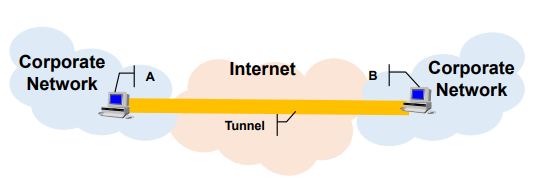
\includegraphics[width=0.90\textwidth]{figure/e2e.png}
            %\caption{qemu-system-arm-version}  
        \end{figure}
    \end{itemize}
    \item Remote VPN tunneling
    \begin{itemize}
        \item Tunnel terminated on end system and VPN gateway
        \begin{figure}[H]
            \centering
            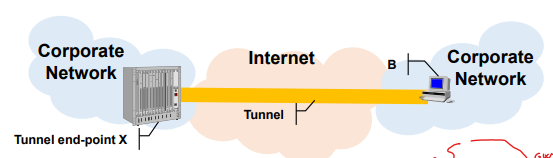
\includegraphics[width=0.90\textwidth]{figure/remote_VPN.png}
            %\caption{qemu-system-arm-version}  
        \end{figure}
    \end{itemize}
Along with the 3 types of VPNs mentioned above, they can also implement 2 types of model (Peer and overlay) that can implements a customer solution or a provider solution each.
\begin{figure}[H]
    \centering
    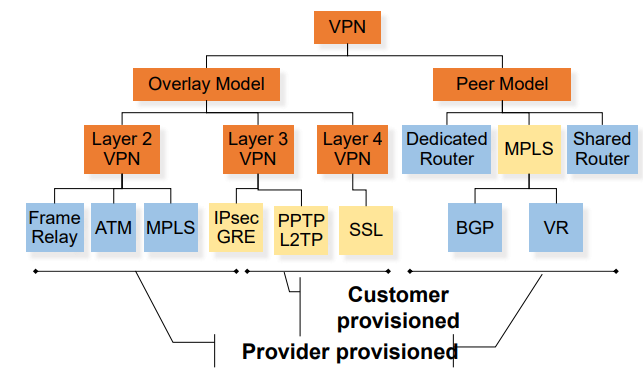
\includegraphics[width=0.90\textwidth]{figure/solutions.png}
    %\caption{qemu-system-arm-version}  
\end{figure}
    \item Overlay model
    \begin{itemize}
        \item The public network does not participate in realizing the VPN (gateways don't interact with router because the first one encapsulate traffic and the second one cannot read the so, the routing is not optimize)
        \begin{itemize}
            \item It does not know where VPN destinations are
            \item just connectivity among VPN gateways
        \end{itemize}
        \item Each VPN gateway must be “in touch” with every other VPN gateway
        \item Routing is performed by the VPN gateways
        \item used when the traffic pass through public internet
    \end{itemize}
    \item Peer model
    \begin{itemize}
        \item Each VPN gateway interacts with a public router (its peer) (gateways interact with router, so the routing is optimize)
        \begin{itemize}
            \item exchange of routing information so we cannot have an end-to-end and we can only apply side-to-side solution
            \item Service provider network disseminates routing information
        \end{itemize}
        \item Public network routes traffic between gateways of the same VPN
    \end{itemize}
    \item Customer provisioned VPN
    \begin{figure}[H]
        \centering
        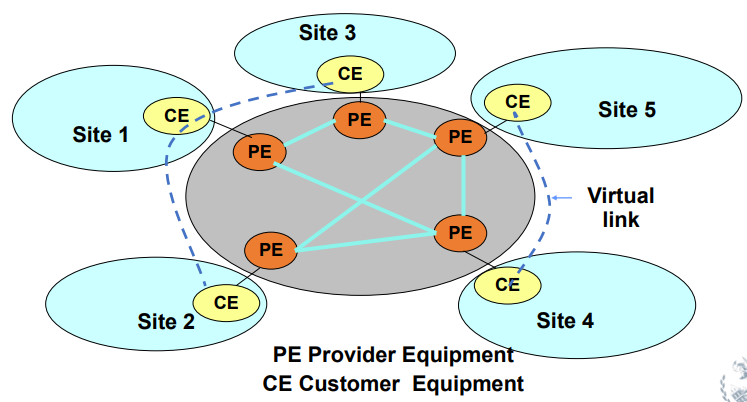
\includegraphics[width=0.90\textwidth]{figure/customer_provisioned_VPN.png}
        %\caption{qemu-system-arm-version}  
    \end{figure}
    \begin{itemize}
        \item the customer owns, configures, manages device implementing VPN functionalities with the use of Customer Equipment (CE)
        \item network provider is not aware that the traffic generated by customer on its VPN
        \item all VPN features implemeted are in the customer device
        \item The CE terminates tunnels
        \item (it isn't possible to have a p2p configuration with a customer model when the traffic has to pass through the internet)
        \item the IP of the gateway is public
        example of remote access VPN customer provisioned:
        \begin{figure}[H]
            \centering
            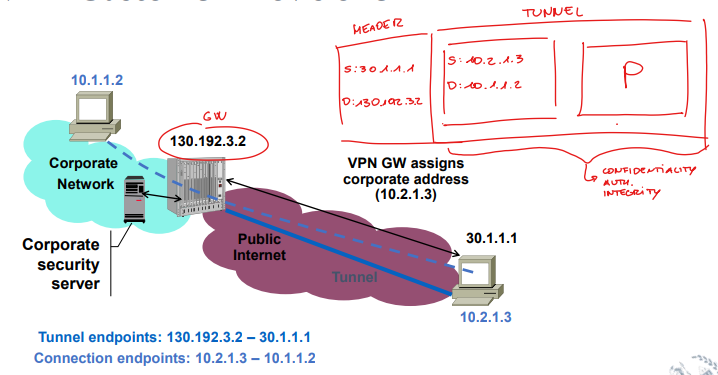
\includegraphics[width=0.90\textwidth]{figure/access_VPN_customer.png}
            %\caption{qemu-system-arm-version}  
        \end{figure}
    \end{itemize}
    \item Provider provisioned VPN (gateway menaged by provider so customer manage the traffic) 
    \begin{figure}[H]
        \centering
        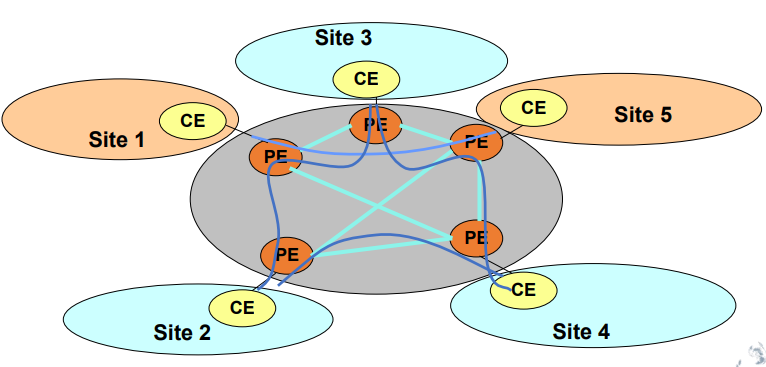
\includegraphics[width=0.90\textwidth]{figure/provider_provisioned_VPN.png}
        %\caption{qemu-system-arm-version}  
    \end{figure}
    \begin{itemize}
        \item the provider owns, configures, manages device implementing VPN functionalities
        \item the provider device maintain the state of VPN
        \item the provider device separates traffic belonging different VPNs
        \item CE may behave as if it were connected to a private network
        \item Provider Equipment (PE) terminates tunnels
    \end{itemize}
    \item differences between customer and provider solution
    \begin{itemize}
        \item customer provisioned (gateway menaged by customer so customer manage the traffic)
        \begin{itemize}
            \item the ISP assign and corporate to a remote host 2 addresses (1 public and 1 private)
            \item remote host terminates VPN tunnel
            \item remote host must active tunnel to permit a client to operate with VPN
            \item Can be used from any internet connection (ISP)
        \end{itemize}
        \item Provider provisioned
        \begin{itemize}
            \item remote host has 1 address (corporate)
            \item NAS terminates VPN tunnel (nas = a device dedicated to store some file and it permits to access to them by a consumer)
            \item Remote host is always on VPN
            \item iternet access is only centralized
            \item Require access to specific ISP
        \end{itemize}
    \end{itemize}
\end{itemize}

\subsection{Virtual VPN topologies}
\begin{itemize}
    \item Hub and spoke (a stella)
    \begin{itemize}
        \item Each branch communicates directly with headquarters
        \item fits to data flow of many corporations
        \item routing is sub-optimal
        \item small number of tunnels
        \item hub could become bootleneck
        \item more simple to create
    \end{itemize}
    \item Mesh (maglia)
    \begin{itemize}
        \item larger number of tunnel so it is more difficult to menage
        \item optimize routing
    \end{itemize}
\end{itemize}

\subsection{Layer and tunneling}
\begin{itemize}
    \item layer 2 VPNs
    \begin{itemize}
        \item Virtual private LAN service
        \begin{itemize}
            \item Emulates functionalities of LANs
            \item Can be used to connect LAN segments that works as a single LAN through the public network
            \item VPN solution emulates learning bridges using routing based on MAC address
        \end{itemize}
        \item Virtual private wire service
        \begin{itemize}
            \item emulates a dedicated line
            \item any protocol can be carried
        \end{itemize}
        \item IP-only LAN-like servie
        \begin{itemize}
            \item CEs are IP routers or IP hosts 
            \item only IP (plus ICMP and ARP) packets travel trough the VPN
        \end{itemize}
    \end{itemize}
    \item layer 3 VPNs
    \begin{itemize}
        \item Protocol used IP (layer 3 address)
        \begin{itemize}
            \item Peer: VPN/corporate address of the local network/customer addresses
            \item Overlay: backbone addresses
        \end{itemize}
        \item Layer 3 packets are forwarded through the public network
        \item CEs are IP routers or IP hosts
    \end{itemize}
    \item tunneling L3 \\\
    a packet (or frame) is carried through an IP network within an IP packet 
    \begin{figure}[H]
        \centering
        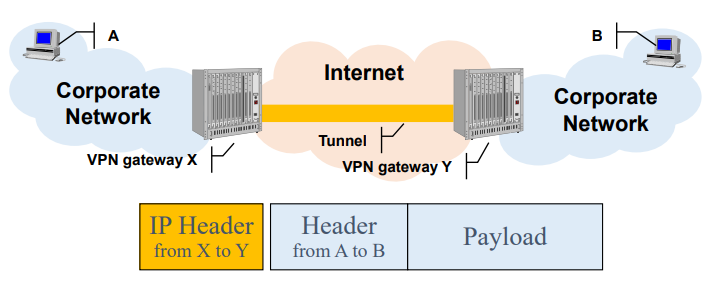
\includegraphics[width=0.90\textwidth]{figure/IP_in_IP_tunnel.png}
        %\caption{qemu-system-arm-version}  
    \end{figure}
    \begin{itemize}
        \item we can add a layer 2 frame (header), within an IP packet (L2TP, PPTP based on GRE)
        \item An IP packet withing an IP packet (IP-in-IP) so we add a IP header to the IP packet
        \begin{itemize}
            \item A and B are corporate addresses (not necessarily public)
            \item tunneling enables communication
            \item Tunneling by itself doesn't ensure security
        \end{itemize}
    \end{itemize}    
    \item Layer 4 VPN
    \begin{itemize}
        \item s2s
        \begin{itemize}
            \item VPN is built using TCP tunnel connections
            \item Security achieved with SSL/TLS
            \item When we add an header of L4, we have to also add a new header at L3 to permit the networking
        \end{itemize}
        \begin{figure}[H]
            \centering
            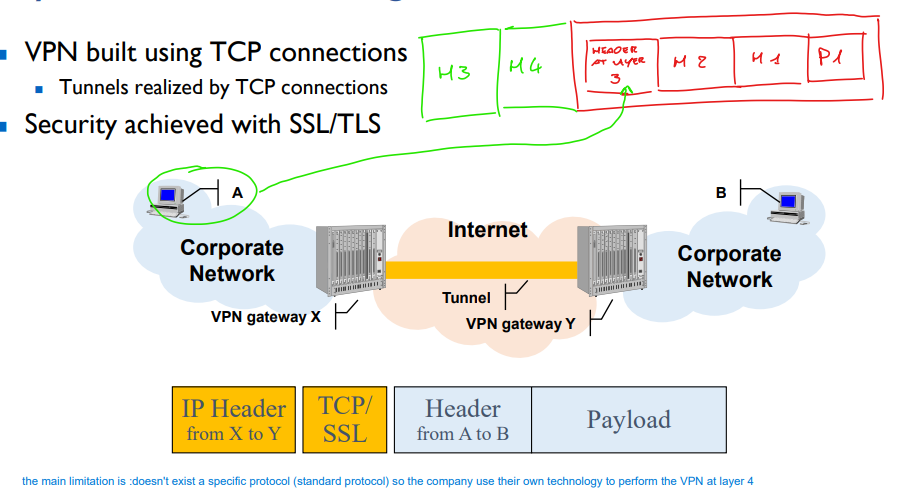
\includegraphics[width=0.90\textwidth]{figure/s2s_layer4.png}
            %\caption{qemu-system-arm-version}  
        \end{figure}
        \item e2e
        \begin{itemize}
            \item Tunnel possibly terminated on end systems
        \end{itemize}
        \begin{figure}[H]
            \centering
            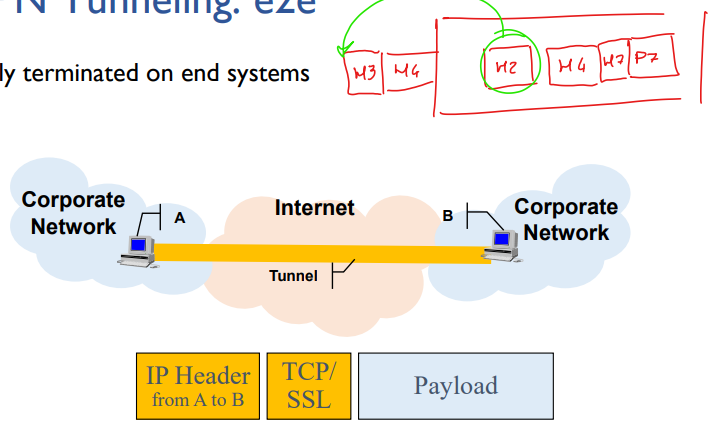
\includegraphics[width=0.90\textwidth]{figure/e2e_layer4.png}
            %\caption{qemu-system-arm-version}  
        \end{figure}
    \end{itemize}
\end{itemize}

\subsection{GRE - generic routing encapsulation}
\textbf{GOAL:} create an encapsulation of any protocol to IP (also IP)
\begin{itemize}   
    \item version 0
    \begin{itemize}
        \item Header fields 
        \begin{itemize}
            \item C, R, K, S are flags that indicate the presence/absence of optional fields
            \item s it indicates "strict source routing flag" and it means that if the destination is not reached when the source route list end, the packet is dropped
            \item Recur that is the max. number of additional encapsulation permitted (must be 0)
            \item protocol where there is the ID of the protocol
            \item Routing which there are the sequence of router IP addresses or ASs for source routing
        \end{itemize}
        \begin{figure}[H]
            \centering
            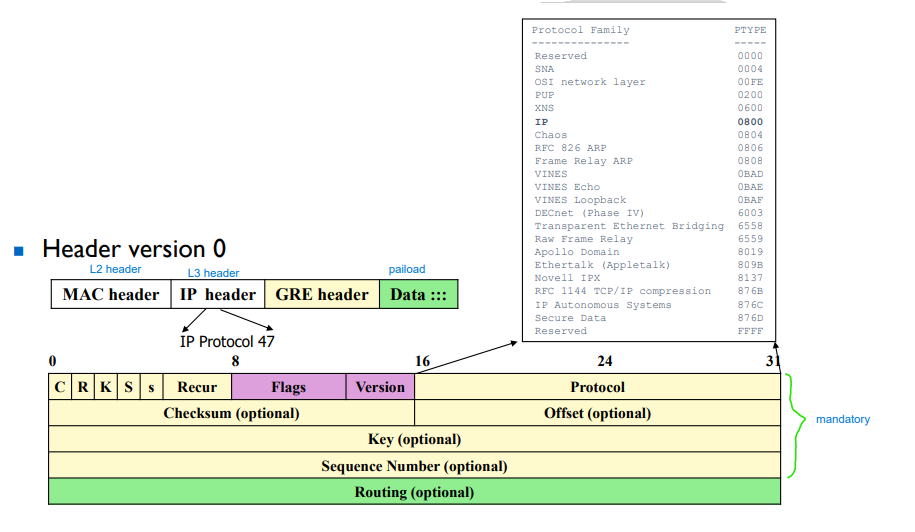
\includegraphics[width=0.90\textwidth]{figure/GRE_header_0.png}
            %\caption{qemu-system-arm-version}  
        \end{figure}
    \end{itemize}
    \item version 1
    \begin{itemize}
        \item Deployed by PPTP
        \begin{itemize}
            \item a key (high 16 bits) to describe the ONLY payload length
            \item a key (low 16 bits) used for the call ID that describe the session ID for this packets
            \item sequence number for ordered delivery, error detection and correction
            \item ACK number (highest number of GRE packet received for this session) to notify the delivery of the packet    
        \end{itemize}
        \begin{figure}[H]
            \centering
            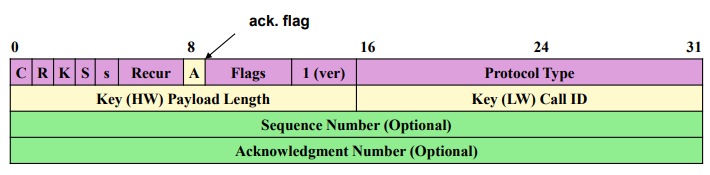
\includegraphics[width=0.90\textwidth]{figure/GRE_header_1.png}
            %\caption{qemu-system-arm-version}  
        \end{figure}
    \end{itemize}
    \item mechanism in GRE
    \begin{itemize}
        \item flow control to slide window mechanism
        \item out-of-order packets that are discarded for the feature of PPP that allow lost packets but cannot handle out of order packets
        \item timeout values re-computed when an ack packet is received
        \item congestion control 
    \end{itemize}
\end{itemize}

\subsection{Layer 2 frame, within an IP packet}
\begin{itemize}
    \item L2TP (Layer 2 Tunneling Protocol)
    \begin{itemize}
        \item Initially only Provider provisioner solition
        \item Idependent of layer 2 protocol on host
        \item Security through IPsec that is strong but complicated
    \end{itemize}
    \item PPTP (Point-to-Point Tunneling Protocol)
    \begin{itemize}
        \item Customer provisioner solution
        \item Originally proposed by Microsoft, Apple, …
        \item Weak encryption and authentication
        \item Proprietary key management
    \end{itemize}
\end{itemize}
\subsection{L2TP - Layer 2 Tunneling Protocol}
\begin{itemize}
    \item user connected with a PPP connection with the LAC and the LAC create a L2 tunnel (L2TP) with the network server (how? first control connection between LAC and LNS and after establish 1 or more session triggered by a call request. after that the tunneling PPP frames is set). the provider offer LAC to the user that permits the tunneling
    \begin{itemize}
        \item peer can be authenticated
        \item a shared secret must exist between LAC and LNS
        \item L2TP uses a CHAP-like mechanism for the auth (Challenge-Handshake Authentication Protocol: A challenge is proposed to the other peer, The correct answer to the challenge requires the shared secret)
        \item The tunnel endpoints exchange the local ID attributed to the tunnel
    \end{itemize}
    \item solution components
    \begin{itemize}
        \item create a tunnel between public network access point (internet service provider)
        \item L2TP access concentrator (LAC) : network access device supporting L2TP and a NAS
        \item L2TP network server (LNS) : corporate VPN gateway       
    \end{itemize}
    \begin{figure}[H]
        \centering
        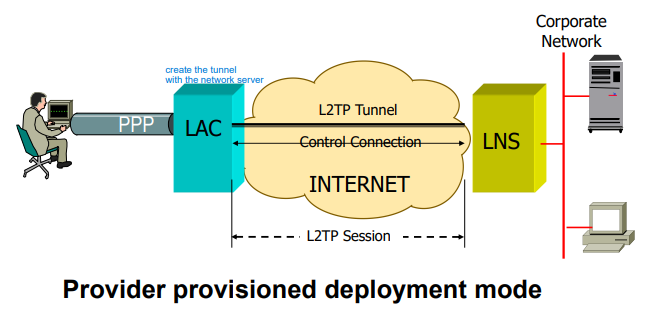
\includegraphics[width=0.90\textwidth]{figure/L2TP.png}
        %\caption{qemu-system-arm-version}  
    \end{figure}
    \item inside the tunnel we can have different session like SSH and for that reason we have a control connection that send only the message for the management of the session.
    \item L2TP header
    \begin{figure}[H]
        \centering
        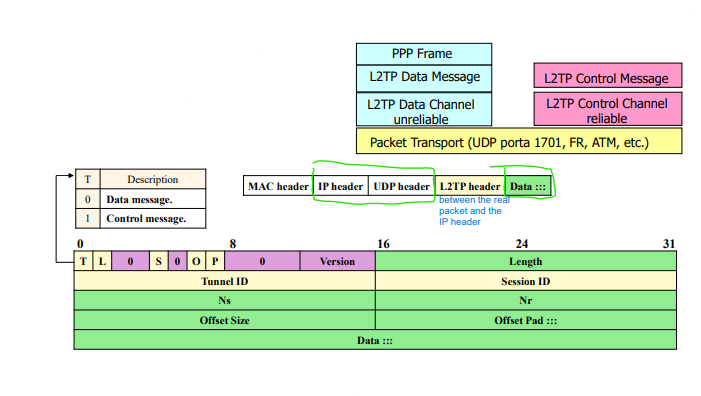
\includegraphics[width=0.90\textwidth]{figure/L2TP_header.png}
        %\caption{qemu-system-arm-version}  
    \end{figure}
    \begin{itemize}
        \item can be a Control message or a Data message
        \item header fields
        \begin{itemize}
            \item L,S,O are some flags
            \item P priority flag
            \item ver version
            \item Tunnel ID id of the control connection
            \item Session ID id of the session within the same tunnel
            \item Ns sequence number of the data or control message
            \item Nr sequence number of the NEXT control message to be received
            \item Offset number of bytes before the beginning of the payload
        \end{itemize}
        \item sequence numbers in data connection is used only to detect out of order packets withouth retransmission and ACK, instead of in the control connection is iused ACK and re-transmission with also the use of the windows set to 32 k
        \item security issues
        \begin{itemize}
            \item Tunnel endpoint authentication
            \begin{itemize}
                \item Authentication only during tunnel establishment phase so an attacker can snoop traffic, can easily inject packets in a session and tunnel and session IDs should be selected in an unpredictable way (not sequentially)
            \end{itemize}
            \item Packet level security
            \begin{itemize}
                \item Encryption, authentication, and integrity must be provided by the transport mechanism like IPsec
            \end{itemize}
            \item End-to-end authentication must be provided by the transport mechanism like IPsec
        \end{itemize}
    \end{itemize}
\end{itemize}
\subsection{PPTP – Point-to-Point Tunneling Protocol}
the customer create a tunnel between its terminal to the specific network service (PNS) that allow to interact with the corporate network. Originally was a proprietary solution but after some years IETF create the standard version
\begin{figure}[H]
    \centering
    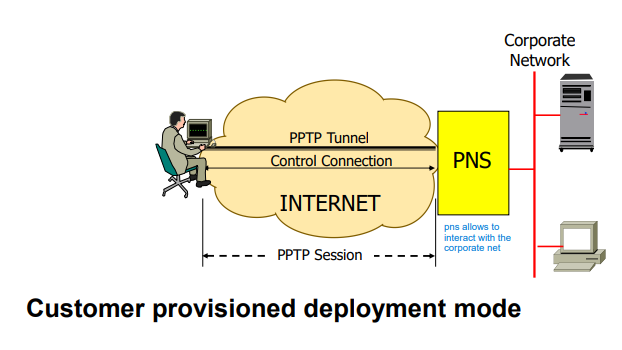
\includegraphics[width=0.90\textwidth]{figure/PPTP.png}
    %\caption{qemu-system-arm-version}  
\end{figure}
\begin{itemize}
    \item General features
    \begin{itemize}
        \item Tuneling of PPP frames over packet switched networks
        \item MPPE (microsoft encryption)
        \item MS CHAP (microsoft auth)
        \item PNS (PPTP network server that is corporate VPN gateway)
        \item PAC (PPTP access concetrator) used for provider provisioned deployment mode
    \end{itemize}
    \begin{figure}[H]
        \centering
        \includegraphics[width=0.50\textwidth]{figure/data_tunneling.png}
        %\caption{qemu-system-arm-version}  
    \end{figure}
    \item PPTP connection
    \begin{itemize}
        \item PPTP data tunneling based on PPP tunneling or GRE protocol
        \item Control connection also supported for the set up and management of the system that is usually based on TCP encapuslation
    \end{itemize}
    \begin{figure}[H]
        \centering
        \includegraphics[width=0.50\textwidth]{figure/control_connection.png}
        %\caption{qemu-system-arm-version}  
    \end{figure}
    \begin{figure}[H]
        \centering
        \includegraphics[width=0.50\textwidth]{figure/PPTP_header.png}
        %\caption{qemu-system-arm-version}  
    \end{figure}
\end{itemize}

\subsection{IPsec VPN}
IPsec is composed by several protocol inside it, 2 are the main protocol that protect the communication (AH, ESP) and another protocol (IKE) that is used to manage the key part and decide the ciphersuite for the protocol.
in the IP sec document is presented:
Authentication Header (AH) that is an extension header to provide message authentication.
Encapsulating Security Payload (ESP) that consists of an encapsulating header and trailer used to provide encryption or combined encryption/authentication.
Internet Key Exchange (IKE) that is a collection of documents describing the key management schemes for use with IPsec (nowadays we use the second version of this protocol).
documents define and describe also cryptographic algorithms for encryption, message authentication, pseudorandom functions (PRFs), and cryptographic key exchange.
IPsec can provides security services at the IP layer like access control, connectionless integrity, data origin auth, rejection of replayed packets, confidentiality and limited traffic flow confidentiality.
\begin{itemize}
    \item The network administrator
    \begin{itemize}
        \item can select the traffic by the quintuple (IP source, IP dest, Port source, Port destination, Protocol type)
        \item which features implement : auth/confiden/auth+confid/null. In the second version can provide confid/auth+confid
        \item which algo use (ciphersuite)
        \item tunnel mode/transport mode 
    \end{itemize}
\end{itemize}
 

\begin{itemize}
    \item security association (AS)
    \begin{itemize}
        \item A key concept that appears in both the authentication and confidentiality mechanisms for IP is the security association (SA).
        \item An association is a one-way logical connection between a sender and a receiver that affords security services to the traffic carried on it, so if a peer relationship is needed for two-way secure exchange, then two security associations are required.
        \item A security association (the logical struct where a netw admin configure the info on the specific tunnel that he would like to create) is uniquely identified by three parameters
        \begin{itemize}
            \item Security Parameters Index (SPI): A 32-bit unsigned integer assigned to this SA and having local significance only. The SPI is carried in AH and ESP headers to enable the receiving system to select the SA under which a received packet will be processed.(rapresent a number that we associate to the AS in order to have an identifier for that specific SA)           
            \item IP Destination Address: This is the address of the destination endpoint of the SA, which may be an end-user system or a network system such as a firewall or router
            \item Security Protocol Identifier: This field from the outer IP header indicates whether the association is an AH or ESP security association.
        \end{itemize} 
    \end{itemize}
    \item security association database (SAD)
    \begin{itemize}
        \item Security Parameter Index (SPI): A 32-bit value selected by the receiving end of an SA to uniquely identify the SA. In an SAD entry for an outbound SA, the SPI is used to construct the packet’s AH or ESP header. In an SAD entry for an inbound SA, the SPI is used to map traffic to the appropriate SA.
        \item Sequence Number Counter: A 32-bit value used to generate the Sequence Number field in AH or ESP headers (required for all implementations). 
        \item Sequence Counter Overflow: A flag indicating whether overflow of the Sequence Number Counter should generate an auditable event and prevent further transmission of packets on this SA (required for all implementations).
        \item Anti-Replay Window: Used to determine whether an inbound AH or ESP packet is a replay (required for all implementations).
        \item AH Information: Authentication algorithm, keys, key lifetimes, and related parameters being used with AH (required for AH implementations).
        \item ESP Information: Encryption and authentication algorithm, keys, initialization values, key lifetimes, and related parameters being used with ESP (required for ESP implementations).
        \item Lifetime of this Security Association: A time interval or byte count after which an SA must be replaced with a new SA (and new SPI) or terminated, plus an indication of which of these actions should occur (required for all implementations).
        \item IPsec Protocol Mode: Tunnel or transport. 
        \item Path MTU: maximum size of a packet that can be transmitted without fragmentation on a specific path and aging variables (required for all implementations). 
    \end{itemize}
    \item Security Policy Database (SPD)
    \begin{itemize}
        \item the binding between IP traffic to a specific SA (contains entries and each defines a subset of IP traffic and a point to a SA for that traffic)
        \item may be multiple entries that are related to a single SA or multiple SAs associated with a single SPD entry
        \begin{itemize}
            \item set of IP and upper-layer protocol field values called selectors define an SPD entry
            \item used to filter outgoing traffic in order to map it into particular SA
        \end{itemize}
        \item Selector
        \begin{itemize}
            \item remote IP address : may be single IP address or range of address, or a wildcard address (these last 2 are required to support more than one destination system sharing the same SA)
            \item Local IP address : description is the same of the remote IP address
            \item next layer protocol : the IP protocol header includes a field that designates the protocol operating over IP
            \item name : user identifier from the operating system
            \item local and remote ports : these may be individual TCP or UDP port values, or a list of ports or a wildcard port
        \end{itemize}
    \end{itemize}


    \item Transport mode (only auth if AH is used)
    \begin{figure}[h]
    \centering
    \includegraphics[width=0.90\textwidth]{figure/transport.png}
    %\caption{qemu-system-arm-version} 
\end{figure}
    \item Tunnel mode (IP header and payload are protected)
    \begin{figure}[h]
    \centering
    \includegraphics[width=0.90\textwidth]{figure/tunnel.png}
    %\caption{qemu-system-arm-version} 
    \end{figure}
    \begin{figure}[h]
    \centering
    \includegraphics[width=0.90\textwidth]{figure/service_protocols.png}
    %\caption{qemu-system-arm-version} 
    \end{figure}
    \item AH
    \begin{itemize}
        \item source auth
        \item data integrity
        \item data origin auth
        \item anti-replay
        \item no confidentiality
        \item AH header insterted between IP header and payload 
        \item routers process datagrams as usual
        \begin{figure}[h]
        \centering
        \includegraphics[width=0.90\textwidth]{figure/AH_packet.png}
        %\caption{qemu-system-arm-version} 
        \end{figure}
        \item SPI gives the session ID and how to verify a signature describing the crypto algo and the reference to key
        \item auth data that store the result of the hash of the original packet and it is considered a crypto signature
        \item new header field which specify the protocol in payload 
        \item protection level of AH
        \begin{itemize}
            \item in trasport mode the entire original packet is authenticated without mutable fields of the packets
            \item in the tunnel mode the entire inner IP packet and the header of the outer packect is authenticated without mutable fields
        \end{itemize}
    \end{itemize}
    \item ESP
    \begin{itemize}
        \item gives data confidentiality of the payload, the ESP trailer and the next header field
        \item host authentication and data integrity
        \item gives authentication from the ESP header to the ESP trailer with the ESP authentication positioned at the end of the packet
        \begin{figure}[h]
        \centering
        \includegraphics[width=0.90\textwidth]{figure/ESP_format.png}
        %\caption{qemu-system-arm-version} 
        \end{figure}
        \begin{figure}[h]
        \centering
        \includegraphics[width=0.90\textwidth]{figure/ESP_packet.png}
        %\caption{qemu-system-arm-version} 
        \end{figure}   
    \end{itemize}
    \item AH and ESP in Tunnel mode and transport mode 
    \begin{figure}[h]
        \centering
        \includegraphics[width=0.90\textwidth]{figure/format_packets.png}
        %\caption{qemu-system-arm-version} 
    \end{figure}
    \begin{figure}[h]
        \centering
        \includegraphics[width=0.90\textwidth]{figure/features_in_differents_case.png}
        %\caption{qemu-system-arm-version} 
    \end{figure}
    \item Combining security association
    \begin{itemize}
        \item in IPsec protocol if i would like to have the combination of AH + ESP i need to have 2 different SA. So multiple SA must be employed for the same traffic flow to achieve the desired IPsec services
        \item There are 2 way to combine different SA
        \begin{itemize}
            \item Transport adjacency: (spiegazione valenza: possibility to have adjency between 2 SA in order to create a unique tunnel). Apply more than one security protocol to the same IP packet without invoking tunneling.            
            \item Iterate tunneling: (spiegazione valenza:possibility to have nested layer, so one layer inside another one). Refers to the application of multiple layers of security protocols effected through IP tunneling
            \item le slides 110 e 111 non sò minimamente cosa voglia spiegare però durante la spiegazione le ha balzate quindi le balzerei
        \end{itemize}
    \end{itemize}
    \item basic combinations of security association 
    \begin{figure}[h]
        \centering
        \includegraphics[width=0.90\textwidth]{figure/basic_comb_SA.png}
        %\caption{qemu-system-arm-version} 
    \end{figure}
    \begin{itemize}
        \item case 1: this is the example of transport adjacency that perform AH+ESP
        \item case 2: it is the typical case that we describe as s2s tunnel, in practice the internet part is considered untrust and for this reason we create a tunnel and we have only 1 tunnel between these 2 gateways. in practice all the traffic or a part of it from this local area network are protected by a SA that create this tunnel.
        \item case 3:we have a combination of an e2e tunnel between the 2 hosts and in addiction we have a s2s between these 2 gateway. why we have this typo of solution? we can have only the integrity for the e2e communication plus confidentiality in the part of the internet that is untrust. Another case is i want a direct protection between the 2 hosts an in addition have what that we call a minimum level of security
        \item case 4: i have a end to end plus a remote access. i have a secure tunnel between the 2 hosts and in addiction i have this level of protection (tunnel SA). how i can create? by 2 SA. 1 for the protection of data between 2 host with an internal tunnel, while the traffic between the host on the left and the gateway can be protected by the other tunnel.
    \end{itemize}
    \item IKE
    \begin{itemize}
        \item IKE implements the following functions
        \item Negotiation of security parameters
        \item Device authentication (source of the traffic)
        \item Key establishment used for the communication (symmetric key)
        \item Key management (after establishment)
        \begin{itemize}
            \item Manual: a system administrator manually configures each system with its own keys and with the keys of the other communicating systems.
            \item Automated: an automated system enables the on-demand creation of keys for SAs and facilitates the use of keys in a large distributed system 
        \end{itemize}
        \item Version 1 (more complicated) and divided in 2 phases
        \begin{itemize}
            \item phase 1: realized in 2 different modes (IKE main mode or IKE aggressive mode) performed by ISAKMP sub-protocol related on the negotiation of a SA between the client and the server. So, in this phase we have the definition of SA, the mutual peer auth and the generation of keys used for the exchange of the IKE message
            \begin{itemize}
                \item first message they would like to decide the list of crypto transform that are supported by the responder and the initiator using an ISAKMP SA proposal
                \item select from the list and return it in the ISAKMP SA response
                \item Then each peer sends a public Diffie-Hellman factor and a nonce which are used to derive encryption and HMAC keys for all further IKE messages. The nonces protect against replay attacks.
                \item where the last exchange of IKE Main Mode is used to confidentially transmit the peer identities, an RSA-signed hash computed over all previous messages and optionally a certificate that can be used by the receiver to verify the RSA signature and with the help of the identity string to authenticate the peer.
                \item the phase 2 is optional and it use IKE Quick Mode. This mode uses three additional messages to exchange the traffic selectors and cryptographic transforms needed for an IPsec SA. Thus the establishment of a single IPsec SA using the IKEv1 protocol requires the exchange of a total of nine UDP datagrams. This fact alone is already reason enough to develop an improved second generation protocol.
                \begin{figure}[h]
                    \centering
                    \includegraphics[width=0.90\textwidth]{figure/IKEV1.png}
                    %\caption{qemu-system-arm-version} 
                \end{figure}
            \end{itemize}
            \item phase 2: implemented by IKE quick mode. Sets up one or several IPsec SAs that produce the ESP keying material required to transmit encrypted and authenticated payload packets.
            \item (IKE use UDP datagrams)
            
        \end{itemize}
        \item Version 2 
        \begin{itemize}
            \item from 9 of the version 1 we use only 4 datagram
            \item employs a strict request/response message exchange scheme with the response always having the function of an acknowledgement. Thus the task of resending messages falls to the initiator. In the case of frequent packet loss or network congestion this consistent scheme makes IKEv2 much more stable than IKEv1
            \item step
            \begin{itemize}
                \item IKE\_SA\_INIT is used to select cryptographic transform for the IKE SA, the derivation of a common Diffie-Hellman secret and the nonces into a single exchange. If Diffie-Hellman public key operation is computationally expensive, the responder can request a coockie if a DOS is suspected 
                \item IKE\_AUTH for the auth of peers using pre-shared keys, RSA signatures, or or the extensible authentication protocol (EAP) but also sets up a first so-called Child SA by defining traffic selectors and the cryptographic transforms for the IPsec connection. As part of the authentication each peer also sends his identity string and optionally a certificate. As a novel feature the initiator may request a the responder to take on a specific identity if the peer is known to possess several.
                \item Multiple Child SAs can be set up by executing the CREATE\_CHILD\_SA request/response pair that carrying the cryptographic transforms, a pair of fresh nonces, an optional DiffieHellman exchange if perfect forward secrecy (PFS) is desired an of course the additional traffic selectors. The CREATE\_CHILD\_SA message exchange is also used for the periodic re-keying of either a Child SA or the IKE SA by including a corresponding notification payload (N)
                \item At any time either peer can send an INFORMATIONAL message which is always acknowledged by a response. An INFORMATIONAL request can contain a notify, a delete SA, or a configuration payload. Empty INFORMATIONAL exchanges can be used to implement Dead Peer Detection (DPD).

                \item spiegazione del prof (sommaria): in the first step the aims of the protocol is to decide the different cryptographic algo in order to share and derive the proper key between the source and the destination. the second step concern having defining the selection crypto transformation and also use DH to decide the key to exchange this information. in the third and fourth in practice the source and the dest encrypt theyr message and in that message are shared info related on the key used or the ESP protocol and AH protocol. This phase is similar like the first one, in practice there are several message like IKE\_AUTH message and the different aspects that are exchanged like cryptographic element. Finally the last phase of the protocol concern the exchange between the initialitator and the responder about the ACK in order to close this type of interaction and notify this phase the selected and the delete SA, in practice in this last phase when all key are establish we have the negotiation of the SA.
            \end{itemize}
        \end{itemize}
    \end{itemize}     
\end{itemize}

\subsection{SSL VPN (layer 4)}
All VPN at layer 4 are based on TLS and they all offer confidentiality.
\begin{itemize}
    \item main architecture TLS based VPN
    \begin{itemize}
        \item s2s VPN
        \item remote access VPN
        \item secure service access
        \item loose interpretation of VPN (SSL pseudo VPN)
        \item tunneling based on TCP or UDP (there is a protocol that is TLS but it doesn't based on TCP like usual but it is based on UDP)
    \end{itemize}
    \item why IPsec is not perfect to use?
    \begin{itemize}
        \item IPsec too difficult and/or too expensive to use securely (Too many options to be configured and managed)
        \item Operates in kernel space so in layer 3 and can makes failures potentially catastrophic and the installation is difficult and risky 
    \end{itemize}
    \item advantage SSL VPN
    \begin{itemize}
        \item low complexity in installation, configuration and management
        \item non-interference with kernel
        \item most widely used for realising VPN
        \item higher, more robust security than IKE
        \begin{itemize}
            \item our packet is composed by h3+h4+h7+p7 and we have 2 possibility to forward packet : 
            IPsec VPN with 2 different options: tunnel and transport mode (i need to select AH or ESP or AH+ESP depending if i would like to protect only the original header at L3 or new header...)
            TLS VPN where the packet is full protected by the VPN at layer 4 (the packet is h4+h3+h4+h7+p7) and for properly send the packet we add an extra header at layer 3 (h3+h4(with TLS and TCP/UDP part inside)+h3+h4+h7+p7)
        \end{itemize}
    \end{itemize}
    \item Pros and cons
    \begin{itemize}
        \item no problem with NAT traversal caused by the no auth of IP header and no encryption of ports as with IPsec ESP 
        \item packets are dropped at a higher level and for the reason that this protocol is based on TCP = we have handshake = DOS attacks
    \end{itemize}
    \item Performance
    \begin{itemize}
        \item IP over TCP cannot delivery a packet after a lost one and this loss leads to a bottleneck with the TCP congestion control
        \item TCP over TCP is unpredictable
    \end{itemize}
    \item Main issue of TLS VPN
    \begin{itemize}
        \item iteroperability
        \item product specific features
        \item Implementation weaknesses
        \item client need to be available on specific platforms 
        \item how TLS VPN is used by a normal client
    \end{itemize}
    \item SSL (pseudo) VPN
    \begin{itemize}
        \item can be the connection between a user to a service or an application clients to an application server instead in the IPsec VPN can be a connection between different hosts or host to network
        \item in Summary TCP or UDP tunneling enable NAT traversal, Packet filter traversal and router traversal. the SSL (pseudo) VPN gives different client solution like web browser
        \item different types based on characteristics
        \begin{itemize}
            \item Network extension that is quite similar to a s2s connectivity
            \begin{itemize}
                \item Open VPN, AEP, F5 Networks ... are some vendors that offer this solution
                \begin{figure}[h]
                    \centering
                    \includegraphics[width=0.90\textwidth]{figure/network_extension.png}
                    %\caption{qemu-system-arm-version} 
                \end{figure}                
            \end{itemize}
            \item SSL'e protocol
            \begin{itemize}
                \item this family is consider pseudo VPN (pseudo because we have a connection between client and server)
                \item in this type of VPN, the original versions of the protocols are put on top TLS and these protocols became secure (protocol over SSL like POP, IMAP, SMTP)
                \item secure application protocols
                \item client and server support is required
                \begin{figure}[h]
                    \centering
                    \includegraphics[width=0.90\textwidth]{figure/SSL_protocol.png}
                    %\caption{qemu-system-arm-version} 
                \end{figure}
            \end{itemize}            
            \item application translation
            \begin{itemize}
                \item we have a intermediate node that have a secure tunnel at L7 and it traslate the native application in HTTPS
                \item native protocol between VPN server and application server and HTTP(S) between VPN server and client
                \item it isn't suitable for all applications 
                \item this communication is simple because the client don't need to know the POP in this example
                \item the server don't know secure application because it is performed by the gateway 
                 \begin{figure}[h]
                    \centering
                    \includegraphics[width=0.90\textwidth]{figure/application_translation.png}
                    %\caption{qemu-system-arm-version} 
                \end{figure}
            \end{itemize}
            \item application proxying
            \begin{itemize}
                \item secure communication is between client and gateway, while the rest of the communication is insecure
                \item we can consider it like the generalization of application translation 
                \begin{figure}[h]
                    \centering
                    \includegraphics[width=0.90\textwidth]{figure/application_proxying.png}
                    %\caption{qemu-system-arm-version} 
                \end{figure}
            \end{itemize}           
            \item port forwarding
            \begin{itemize}
                \item another example more sofisticated of the application proxying is this
                \item in this case we also allow change the specific port in the communication between client and the intermediate gateway for several reason like for not use the default port changing port identifier
                \item we can consider it like the generalization of application translation 
                \begin{figure}[h]
                    \centering
                    \includegraphics[width=0.90\textwidth]{figure/port_forwarding.png}
                    %\caption{qemu-system-arm-version} 
                \end{figure}
            \end{itemize}            
            \item web proxying
        \end{itemize}
    \end{itemize}    
\end{itemize}

\subsection{VPN Gateway Positioning}
\begin{itemize}
    \item VPN gateway and Firewall
    \begin{figure}[h]
        \centering
        \includegraphics[width=0.90\textwidth]{figure/VPN_and_firewall.png}
        %\caption{qemu-system-arm-version} 
    \end{figure}
    \begin{itemize}
        \item inside
        \begin{itemize}
            \item no inspection of VPN traffic because we cipher the plaintex before it is inspected BUT THI PROBLEM IS PERSISTENT BOTH THE DIRECTION FROM IN TO OUT AND VICEVERSA
            \item VPN gateway protected by firewall
        \end{itemize}
        \item parallel
        \begin{itemize}
            \item potential uncontrolled access
        \end{itemize}
        \item outside
        \begin{itemize}
            \item VPN gateway protected by access router
            \item consistent policy
        \end{itemize}
        \item integrated
        \begin{itemize}
            \item maximum flexibility
        \end{itemize}
        \begin{itemize}
            \item 
        \end{itemize}
    \end{itemize}
    \item IPsec, VPN Gateways and NATs
    \begin{itemize}
        
        \item the issue releated to the NAT is that it changes the content of the IP source address and in term of integrity the checksum fail (AH) and the packet is discarded.
        \item in term of encapsulation the source and dest tunnel can be change and for that reason the packet is discarded (ESP)
        \item the same problem occurs for NAT but also for NAPT (NAT that not change the IP address but change the source port). 
        \item the ports are not visible in trasport mode 
        \item another issue concerning the tunnel mode is that in this case i can have the same address for 2 different VPN sites. in tunnel mode if there is a NAT i'm not able to distinguish if some source arrives from Gateway1 or Gateway2 because both are NATTED
        \item in general also the NAT can be put before the gateway = nat - FW - GW - FW
    \end{itemize}
    \item VPN gateway and IDS
    \begin{itemize}
        \item IDS is usually outside the firewall
        \item no control on VPN traffic
        \item multiple IDS sensor
        \begin{itemize}
            \item outside FW
            \item inside VPN gateway
        \end{itemize}
        \begin{figure}[h]
        \centering
            \includegraphics[width=0.90\textwidth]{figure/VPN_and_IDS.png}
            %\caption{qemu-system-arm-version} 
        \end{figure}
    \end{itemize}
    \item Anomaly
    \begin{itemize}
        \item when we don't have a e2e solution and the path is divided in several tunnel we call it \textbf{Monitorability anomaly}. It is when some nodes at the channel junctions can "see" the exchanged data. an attacker can attack the middle nodes and sniff/modify data.
        \begin{figure}[h]
        \centering
            \includegraphics[width=0.20\textwidth]{figure/monitorability_anomaly.png}
            %\caption{qemu-system-arm-version} 
        \end{figure}
        \item \textbf{skewed channel anomaly} is when a wrong tunnel overlapping removes the confidentiality in a part of the communication. Lo spiego in italiano: partiamo dall'immagine qui sotto, nella configurazione abbiamo un remote access tra Ca1 e Gc1 e poi un s2s da ga1 a gc3. nella figura manca ma dobbiamo supporre che ci sia un client Cc3 all'estrema destra. Partendo dall'inizio il paccketto che parte da Ca1 e deve arrivare a Cc3 viene "imbustato" e la source rimane invariata, però la destinazione sarà Gc1. Il pacchetto però in Ga1 verrà imbustato per percorrere la s2s di conseguenza la source diventerà Ga1(dove è tutt'ora il pacchetto) e la destinazione diventerà Gc3. così facendo il gateway Gc1 non potrà fare nulla e solo quando il pacchettò sarà arrivato a Gc3 si avrà la possibilità di spacchettare dal s2s. Arrivati qui il gateway leggerà la destinazione del primo impacchettamento perciò forwarderà quest'ultimo al gateway destinazione (Gc1) che lo spacchetterà e leggerà che la destinazione è Cc3 però arrivati qui il pacchetto da Gc1 a Cc3 viaggerà in cleartext. 
        \begin{figure}[h]
        \centering
            \includegraphics[width=0.90\textwidth]{figure/skewed_channel.png}
            %\caption{qemu-system-arm-version} 
        \end{figure}
        
    \end{itemize}
\end{itemize}

\subsection{CLoud Computing Security}
If designed appropriately, cloud computing causes no more threat to security than what exist in traditional computing. Some security working groups are NIST, CSA, ISO, ETSI... and the technologies that are used to deploy Cloud Computing Security are Amazon Web Service, Google Cloud Platform, K8s ... 
\begin{itemize}
    \item Cloud security model : sort of overview to model and define the different types of protection of cloud.
    \begin{itemize}
        \item NIST cloud business model: rappresent different models of delivery of cloud Software as a service, Platform as a service, infrastructure as a service and also the different type of development models like public cloud, private cloud, community cloud and hybrid cloud.
    \end{itemize}
    \item Cloud Cube Model
    \begin{itemize}
        \item loud Cube Model was originally resolve the issue of deperimeterization network (si riferisce alla tendenza crescente delle organizzazioni a spostarsi da un approccio di sicurezza perimetrale tradizionale a un modello più distribuito e senza confini definiti. Tradizionalmente, la sicurezza di rete si basava su un perimetro ben definito, spesso protetto da firewall, per impedire l'accesso non autorizzato e proteggere i dati e le risorse aziendali. Tuttavia, con l'aumento dell'uso del cloud computing, del lavoro remoto e dei dispositivi mobili, questo perimetro sta diventando sempre più difficile da definire e proteggere.) using \textbf{three-dimensional cube}
        \item it collects all different combinations available in cloud offerings and presents 4 criteria to differentiate various types of cloud formations.
        \item it helps to understand  how security issues can be approached in cloud computing
        \item objectives
        \begin{itemize}
            \item different formations of clouds
            \item highlight their key characteristics
            \item represent benefits and risks
            \item present a roadmap to make the environment more secure
        \end{itemize}
        \item Design 4 criteria that make 16 different forms of cloud computing environment
        \begin{enumerate}
            \item physical storage location (Data Boundary: Internal / External)
            \begin{itemize}
                \item For example, virtualized hard disks in an organization’s data center would be internal, while Google Cloud Storage would be external at some location “off-site”
                \item a false assumption is that internal is more secure than external
            \end{itemize}
            \item cloud is formed by using proprietary technology or open technology(Ownership: Proprietary / Open)
            \begin{itemize}
                \item it indicates the degree of interoperability and data/application transportability between your own systems and other cloud forms, and the ability to withdraw your data from a cloud form or to move it to another without constraint.
                \item if it is proprietary, the organization that provides service also maintain the provision under its ownership
                \item if it is proprietary, you may not be able to move to another cloud supplier without significant effort or investment
                \item proprietary services don't collaborate with other service withouth agreement and this provides an isolate/secure environment
                \item often the more innovative technology advances occur in the proprietary domain.
                \item open can easily collaborate with all other open clouds
                \item open cloud service are built following open standards
            \end{itemize}
            \item the cloud will operate outside the boundary of the organization's network or only inside (Security Boundary: Perimeterized / De-perimeterized)
            \begin{itemize}
                \item traditional network boundaries are indicates by firewalls
                \item more security but less collaboration because it doesn't allow other systems to access anything inside its own perimeter.
                \item VPN expands the network boundary but keeps the computing environment perimeterized during collaboration as it uses local networking protocols
                \item de-perimeterized system shows the intent to collaborate with systems outside (Collaboration Oriented Architecture) but should be protected by using techniques like data level auth, encryption ecc
            \end{itemize}
            \item the development and maintenance of cloud service is done in-house team or outsourced (Sourcing: Insourced / Outsourced)
            \begin{itemize}
                \item The service sourcing is not a technical issue rather it is basically a business decision.
                \item insourced service = private cloud
                \item outsourced service = public and private cloud
                \item the sourcing decision must take care of the expertise and reputation of the team that is going to deliver the cloud.
            \end{itemize}
            \begin{figure}[h]
                \centering
                \includegraphics[width=0.90\textwidth]{figure/cloud_cube_model.png}
                %\caption{qemu-system-arm-version} 
            \end{figure}
        \end{enumerate}
    \end{itemize}
    \item cloud responsibility
    \begin{itemize}
        \item The security issues associated with cloud computing can be viewed from two angles: as the concerns of cloud providers (providing SaaS, PaaS or IaaS) and the concerns of the service consumers
        \begin{itemize}
            \item The provider must ensure security of its own infrastructure
            \item The consumers must verify and make sure that the provider has employed all possible security measures to make the services secure
            \begin{figure}[h]
                \centering
                \includegraphics[width=0.90\textwidth]{figure/cloud_responsibility.png}
                %\caption{qemu-system-arm-version} 
            \end{figure}
        \end{itemize}
    \end{itemize}
    \item Service Level Agreements (SLA)
    \begin{itemize}
        \item used in different industries to establish a trust relationship between service providers and consumers
        \item it details the service-level capabilities promised by the providers to be delivered and requirements/expectations stated by consumers
        \item document establishes a legal binding for both the parties and works as reference in any dispute
        \item consumer has to establish (in some cases) and verify the requirements
        \item CyberSecurity SLA 
        \begin{itemize}
            \item more in detail SLA document should include the security issues in adequate detail
            \item maintenance activities need to define the responsibilities of both service providers and consumers in documented form
            \item should have detailed mentioning of the security capabilities of the solutions and the security standards to be maintained by the service providers.
            \item Consumers, on the other hand, should provide clear-cut information to the service providers about what they consider as a breach in security.
        \end{itemize}
    \end{itemize}
    \item Cloud Computing Threats = A threat in the Cloud is a potential (or actual adverse) event that may be malicious or incidental (i.e. failure of a storage device), compromising Cloud resources
    \begin{figure}[h]
        \centering
        \includegraphics[width=0.90\textwidth]{figure/cloud_threats.png}
        %\caption{qemu-system-arm-version} 
    \end{figure}
    % \begin{itemize}
    %     \item Different service delivery/receiving model
    %     \begin{itemize}
    %         \item organizations need to evaluate the risks associated with the loss of control over the infrastructure.
    %         \item it is important also where i store data Data because traversing over geographical boundaries are subjected to different federal laws
    %     \end{itemize}
    %     \item Abuse and nefarious use of cloud
    %     \begin{itemize}
    %         \item cloud computing provides bandwidth and storage capacities and vendors don't have sufficient control over the attackers, malicious users or spammers that can take advantages of the trials and these can often allow an intruder to plant a malicious attack and prove to be a platform for serious attacks
    %         \item for protection: stronger authentication and the user’s network traffic should be monitored comprehensively
    %     \end{itemize}
    %     \item Insecure interface and API
    %     \begin{itemize}
    %         \item Cloud providers often publish a set of interfaces and APIs to allow their customers to design an interface for interacting with Cloud services. These interfaces often add a layer on top of the framework, which in turn would increase the complexity of Cloud and this can allow vulnerabilities by the improper use of it.
    %         \item for protection : use a proper security model for Cloud provider's interface, strong auth and encrypted transmission
    %     \end{itemize}
    %     \item Malicious insiders
    %     \begin{itemize}
    %         \item the attacker is inside 
    %         \item protection: least priviledge 
    %     \end{itemize}
    %     \item Shared technology issues in multi-tenancy environment
    %     \begin{itemize}
    %         \item In multi-tenant architecture, virtualization is used to offer shared on-demand services 
    %         \item Vulnerabilities in a hypervisor allow a malicious user to gain access and control of the legitimate users’ virtual machine
    %         \item protection: Implementation of SLA for patching, strong authentication, and access control to administrative tasks
    %     \end{itemize}
    %     \item Data loss and leakage
    %     \begin{itemize}
    %         \item data may be compromised or stolen in many ways because data are shared and dynamically stored. also with a weak encryption algorithm, or weak keys or don't have a strong auth ...
    %         \item protection : data integrity, secure storage, data backup
    %     \end{itemize}
    %     \item Service/account hijacking
    %     \begin{itemize}
    %         \item the client may redirect to a harmful website using techniques like fraud, phishing ... and if an attacker can access someone's credentials, they can capture the activities, transaction data, manipulate data, return falsified information or redirect the client to illegitimate sites and the hacked account
    %         \item protection : security policy, strong auth and activity monitoring
    %     \end{itemize}
    %     \item risk profiling
    %     \begin{itemize}
    %         \item 
    %     \end{itemize}
    %     \item identity theft
    %     
    % \end{itemize}
    \item Vulnerability 
    \begin{itemize}
        \item the weakness/loopholes in the security architecture of Cloud, which can be exploited by an adversary via sophisticated techniques to gain access to the network and other infrastructure resources.
    \end{itemize}
    \item Cloud Security Issue
    \begin{figure}[h]
        \centering
        \includegraphics[width=0.90\textwidth]{figure/cloud_security_issue.png}
        %\caption{qemu-system-arm-version} 
    \end{figure}
    \begin{itemize}
        \item Data storage and computing security issues
        \begin{itemize}
            \item Loss of control of data is a major issue in cloud computing model because it doesn't provides full control over the data and it is harder to check data integrity and confidentiality. This can be a consequence of the provider that store data on the basis of multi-location (security threats and legal problem) or that the customer of the cloud is physically separated from his data.
            \begin{itemize}
                \item Data storage services(Software as a service), like Dropbox and Google Drive, opt to offer persistent hard storage plans for data
                \item Data that are stored are isolated, inscrutable to the customers, consistent during computation and cannot be modify by someone else.
            \end{itemize}
            \item cloud services need to be up and have a high availability goal
            \begin{itemize}
                \item Providers use a multi-tier architecture, made at the application and infrastructural levels to add high availability and scalability. This approach enable DoS attaks resiliency
                \item At a certain point, resources might be denied to other customers. Nevertheless, such issue is partially blocked by the elasticity feature of cloud environments
                \item availability concern also the HW side. Thus, outage events should be negotiated upfront in SLAs to discriminate disaster recovery and backup plans.
            \end{itemize}
            \item Cryptography mechanism 
            \begin{itemize}
                \item it is the most straightforward security measures applied but it must be careful applied (brute force attacks and the evolving technology for password cracking methods are available to attack)
                \item  Computers pack greater processing power distributed across various platforms, including multi-core CPUs and Graphics Processing Units (GPUs) with high clock rates
                \item 
            \end{itemize}
            \item Sanitization
            \begin{itemize}
                \item \textbf{Sanitization} is the process of cleaning or removing certain pieces of data from a resource after it becomes available for other parties
                \item \textbf{Data sanitization} is an important task in order to properly dispose of data and physical resources that are sent to the garbage.
                \begin{enumerate}
                    \item Deficient implementation of data destruction policies at the end of a lifecycle, may result in data loss and data disclosure, because hard disks might be discarded without being completely wiped or  might be possible for subsequent tenants to read data previously written.
                \end{enumerate}
            \end{itemize}
            \item Malware (the main problem is that the malware can spread across the cloud or it spreads to all the device which are synchronized with the file it attaches to)
        \end{itemize}
        \item Virtualization security issues
        \begin{itemize}
            \item Development of cloud service for business purpose, cloud provider require trust on VM
            \item there is a problem given by the multi-tenancy
            \item VMs image management
            \begin{itemize}
                \item The dynamic nature of the cloud allows the provider to create, modify and copy VM images.
                \item there lots of security risks from the prospective of the repository administrator, cloud provider and cloud user:
                \begin{enumerate}
                    \item The administrator risks are hosting and distributing malicious images that cause:
                    \begin{enumerate}
                        \item Theft and Code Injection
                        \begin{enumerate}
                            \item Image files have to be kept in a repository which, even at an offline state, are vulnerable to theft and malicious code injection
                            \item protection:concatenate several images, because it is harder to copy large-sized files combined than one only
                        \end{enumerate}
                        \item Unknown vulnerability
                        \item  VM sprawl
                        \begin{enumerate}
                            \item VMs is continuously growing, while most of them are idle or never resumed from sleep, which may cause wasting resources and complicate VMs management
                        \end{enumerate}
                    \item cloud provider risks leaking data if unwittingly publishes images, because images contain fully configured applications and data.
                    \item The cloud user risks is running vulnerable and wrongly administrated repository
                    \end{enumerate}
                \end{enumerate}
                \item If the control of VMM or hypervisor is under the attacker. (Hyperjacking). The attacker can monitor other virtual machines, access the shared infrastructure, monitor the CPU utilization or can bring the VMM shutting down. 
            \end{itemize}
            \item Mobility, 3 main types of issue
                \begin{enumerate}
                    \item Network attack on VMs migration
                    \item Redundancy of erroneous configurations
                    \item Proprietary Information disclosure
                \end{enumerate}
            \item issues in VM (before issues are releated to the MENAGEMENT of VM) reletaed only to the IaaS
            \begin{itemize}
                \item VM hopping : an attack is take access to different VMs belonging to other customer by exploring the VM-to-VM or VM-to-VMM
                \item the successful attack gives various security issues like checking resource usage, alter the configuration of the system and files or the leakage of sensitive data 
                \begin{figure}[h]
                    \centering
                    \includegraphics[width=0.90\textwidth]{figure/VM_hopping.png}
                    %\caption{qemu-system-arm-version} 
                \end{figure}
            \end{itemize}
            \item Malware (The virtualization and sandboxing technique in the cloud provides various advantages, but this is ongoing challenge )
        \end{itemize}
        \item Network security issues
        \begin{itemize}
            \item in order to connect the cloud infrastructure we need to have network infrastructure
            \item the difference between network security issues in a traditional architecture and a cloud environment is the lifecycle of the system. In a cloud environment the modification of links (main part of network) is more frequent because it is a dynamic network.
            \item keywork : \textbf{Security automation and adaptations}
        \end{itemize}
        \item Internet and services related security issues 
        \begin{itemize}
            \item Cloud infrastructures are not only composed by the hardware where the data is stored and processed, but also by the path to where it gets transmitted
            \item Internet is normally used as the transmission medium; one has to assume it's unsafe and inherent problems.
        \end{itemize}
        \item Internet protocols
        \begin{itemize}
            \item TCP/IP model is the basis for communicating in the internet and its issues are still in a web-based environment that use it. For ex DHCP,IP along with DNS may enable network based corss-tenant attacks.
            \item Certain Web sites implement HTTPS in sensitive forms, like a login form, and then the rest of the session is maintained over HTTP (application level not only layer 3 or 4)           
        \end{itemize}
        \item service availability
        \begin{itemize}
            \item attention to DoS attacks
            \begin{itemize}
                \item \textbf{Direct DoS} attacks imply a predetermination of the target service host machine
                \item Possible collateral damage consists in denying other services being hosted on the same machine or network, therein creating \textbf{indirect DoS}.
            \end{itemize}
            \item a proper link bandwitdth is required to support great amout of net traffic
            \item 3 scenarios are possible
            \begin{enumerate}
                \item DDoS attack to the servers
                \begin{enumerate}
                    \item The server overloads by either processing a single malicious request that expects to exploit a vulnerability or processing a massive number of requests
                \end{enumerate}
                \item DDoS attack to the network
                \begin{enumerate}
                    \item A network link is fully saturated with bogus requests belonging to the attack and thus reaches its bandwidth capacity, ceasing honest connections.
                \end{enumerate}
                \item DDoS attack to an intermediate network device (more difficult to define)
                \begin{enumerate}
                    \item One or more intermediate network device (e.g., routers, DNS Resolver, Load Balancer) also become saturated to a large amount of bit rate processing per second (isolate the legitimate user)
                \end{enumerate}
            \end{enumerate}
        \end{itemize}
        \item Access control issues (protection from unauthorized read/write permissions.)
        \begin{itemize}
            \item authentication mechanism
            \item authorization mechanism
            \item To solve this issue, it is important to separate and provide different authorization to each component either logical or physical from one another. 
            \item physical access 
            \begin{itemize}
                \item Data centers centralize massive amounts of data in a single point. Because this data is not owned by the provider, but by a diverse number of heterogeneous customers that outsource their businesses, it can be possible that someone can retrieve any kind of useful sensitive information.
                \item The ultimate goal is to protect information in long-term in a co-habitat like cloud environments
                \item It is crucial to guarantee physical security in order to prevent any kind of data leakage by exploring the wide cloud attack vector from an inside position
                \item money mules are some corrupted employ that are used by a third party company in order to acquire info data, news, important aspects related to a company or make attacks to the company to create problems related reputation.
            \end{itemize}
            \item User credential that if are compromised, it is possible to monitor or manipulate data and transactions, along with performing malicious redirects
            \item anonymization
            \begin{itemize}
                \item it is important that the data of a customer are collected but when are stored this data are anonymized.
                \item The anonymization system provides facility-identity information of the cloud customer should be hidden and not be disclosed in front of any other person
                \item There are deanonymization attack, active attack, and passive attack those can breach user privacy on the basis of user origin knowledge
            \end{itemize}
        \end{itemize}
    \end{itemize}
    \item Cloud protection (main security principles: zecurity by design, zero trust, open deisgn priciple)
    \begin{itemize}
        \item def by NIST: The guidelines provides an overview of the security and privacy challenges facing public cloud computing and presents recommendations that organizations should consider when outsourcing data, applications and infrastructure to a public cloud environment. The document provides insights on threats, technology risks and safeguards related to public cloud environments to help organizations make informed decisions about this use of this technology. 
        \begin{itemize}
            \item key guidelines
            \item plan the security and privacy aspects
            \item Understand the public cloud computing environment offered
            \item Ensure that a cloud computing solution satisfy organizational security and privacy requirements.
            \item Maintain accountability over the privacy and security of data and applications
        \end{itemize}
        \item Governance
        \begin{itemize}
            \item design proper policy, procedures and standard used for the application, different design, different implementation, testing, use and monitoring to deploy services, put in place audit mechanism
        \end{itemize}
        \item Compliance
        \begin{itemize}
            \item understand different lows and regulation that impose security and privacy particularly those involving data location, privacy and security controls, records management and electronic discovery requirements
        \end{itemize}
        \item Trust
        \begin{itemize}
            \item have the guarantee that the cloud provider can be offer service to the customer in the right way establing clear, exclusive ownership right over data
            \item Continuously monitor the security state of the information system
        \end{itemize}
        \item architecture
        \begin{itemize}
            \item Understand the underlying technologies that the cloud provider uses to provision services, including the implications that the technical controls involved have on the security and privacy of the system
        \end{itemize}
        \item Identity and access management
        \begin{itemize}
            \item Ensure that adequate safeguards are in place to secure authentication, authorization and specific techniques for the identity and access management
        \end{itemize}
        \item Software isolation
        \begin{itemize}
            \item all characteristic of multitenant software architecture, and assess the risks involved for the organization
        \end{itemize}
        \item Data protection
        \begin{itemize}
            \item Evaluate the suitability of the cloud provider’s data management solutions for the organizational data concerned and the ability to control access to data, to secure data while at rest, in transit, and in use, and to sanitize data
        \end{itemize}
        \item Availability
        \begin{itemize}
            \item which type of strategy for backup, fast recovery, definitions of a proper service level agreement for data and service availability
        \end{itemize}
        \item Incident response
    \end{itemize}
    \item Security as a service
    \begin{itemize}
        \item  generally meant a package of security services offered by a service provider that offloads much of the security responsibility from an enterprise to the security service provider.
        \item it is a segment of the SaaS offering by a cloud provider
        \item SecaaS characteristics
        \begin{itemize}
            \item it is avilable on-demand and over the net
            \item resources are available for many customer at the same time
            \item elastically (more or less based on the client)
            \item use more pay more and use less pay less
        \end{itemize}
        \item SecaaS advantage
        \begin{itemize}
            \item cost
            \item easy to manage
            \item scalability
            \item fast provisioning
            \item best solution on the market
            \item continuous updates
            \item cost-effective compliance
        \end{itemize}
        \item SecaaS categories
        \begin{itemize}
            \item Identity and access management (auth and author mechanism)
            \item Data loss prevention (mitigation and recovery strategy releated to data)
            \item Web security (as Web application FW)
            \item E-mail security (antispam, and deep packet inspection)
            \item Security assessments
            \item Intrusion management
            \item Security information and event management (alert menagement)
            \item Encryption (of data)
            \item Business continuity and disaster recovery
            \item Network security (packet filter, IDS)
        \end{itemize}
        \item AWS IAM (Identity and access management)  is a web service that helps you securely control access to AWS resources
        \begin{itemize}
            \item it has 2 main tasks:
            \item authentication mechanism (different auth...)
            \item authorization (most difficult to manage)
        \end{itemize}
        \item AWS WAF (web applic firewall)
        \begin{itemize}
            \item protec by:
            \begin{itemize}
                \item SQL injection 
                \item Cross-site scripting 
                \item Http Floods
                \item Scan and probes
            \end{itemize}
            \item different fields:
            \begin{itemize}
                \item IP Match Condition (filter at L3)
                \item Geo Match Condition
                \item String Match Condition (filter at L7)
                \item Regex Condition (Optional) (filter at L7)
                \item SQL Injection Match Condition
                \item Size constraint conditions
                \item Cross-site scripting match conditions
                \item geolocalization condition (block a pecific traffic from a specific place)
            \end{itemize}
            \item it offers only Deny and allow list but it doesn't provide support for the priority of the rules (because without priority is not possible having anomaly in term of conflict, there is only sub optimization than is impossible with an allow list or deny list for an administrator creates conflict anomaly that generates unespected behaviour)
        \end{itemize}
        \item IBM Cloud Security Managed Services provide
        \begin{itemize}
            \begin{figure}[h]
                \centering
                \includegraphics[width=0.90\textwidth]{figure/IBM_cloud_security_managed.png}
                %\caption{qemu-system-arm-version} 
            \end{figure}
            \item Mail security features
            \begin{itemize}
                \item Antivirus
                \item Antispam
                \item Content control for email
                \item Flooding preventions (avoid storm attack)
                \item Image control for email (block image inappropriate)
            \end{itemize}
            \item Web security features
            \begin{itemize}
                \item Antivirus and anti-spyware for web
                \item URL filtering for web
            \end{itemize}
        \end{itemize}
        \item Security and data risk platform (typically it ia a unique security management platform for)
        \begin{itemize}
            \item Assets
            \item vulnerabilities
            \item Threats
            \item Attack Detections
            \item Policies
            \item IAM
            \item Security/risk 
            \item Prioritization
            \item Investigations
            \item a sort of dashboard that allow the security amministrator have awearness of the security level of your system
        \end{itemize}
    \end{itemize}
    \item Compliance
    \begin{itemize}
        \item it spread over multiple countries and all of those different regions are likely to have different regulatory requirements. In cloud computing, becomes necessary to observe how all of these overlapping regulatory requirements are being maintained by the service provider in a coherent manner
        \item what is expected from my infra releated preformance, security and legal compliance
        \item Compliance agreements can be made between a CSP and service consumers through SLA contract
        \item managing compliance issues is done by consumer and the provider
        \item audit and monitoring : audit is the process once a time that offline in a specific time period analyze in depth system  performance, security controls, information privacy, compliance ecc, monitoring is also a regular activity that keep track on all activities performed everyday and on the system, such as intrusion detection and others 
        \begin{figure}[h]
            \centering
            \includegraphics[width=0.90\textwidth]{figure/external_internal_audit.png}
            %\caption{qemu-system-arm-version} 
        \end{figure}
    \end{itemize}
\end{itemize}

\subsection{Network Security Monitoring}
\begin{itemize}
    \item Security Event Logging
    \begin{itemize}
        \item \textbf{Security event}: an accurrence that have potential security implications to a system or its environment
        \begin{itemize}
            \item Logging an operator into or out of the system
            \item Performing a cryptographic operation, such as signing a digital certificate or certificate revocation list
            \item Performing a cryptographic card operation (creation, insertion, removal, or backup)
            \item Performing a digital certificate life cycle operation (rekey, renewal, revocation, or update)
            \item Posting a digital certificate to an X.500 directory
        \end{itemize}
        \item \textbf{Security incident}: An occurrence that actually or potentially jeopardizes the confidentiality, integrity, or availability of an information system.
        \begin{itemize}
            \item Receiving a key compromise notification
            \item Receiving an improper certification request
            \item Detecting an alarm condition reported by a cryptographic module
            \item Failing a built-in hardware self-test or a software system integrity check
        \end{itemize}
        \begin{figure}[h]
            \centering
            \includegraphics[width=0.90\textwidth]{figure/security_event_logging.png}
            %\caption{qemu-system-arm-version} 
        \end{figure}
        \item Objectives
        \begin{itemize}
            \item the objective is e to help identify threats that may lead to an information security incident, maintain the integrity of important security-related information, and support forensic investigations.
            \item With logging is possible to see interactions, and changes that are relevant to security
            \item  record of events such as anomalies, unauthorized access attempts, and excessive resource usage, an enterprise can perform an analysis to determine the cause.
        \end{itemize}    
        \item Security Log Sources
        \begin{itemize}
            \item Server and workstation operating system logs
            \item Application logs (for example, web server, database server)
            \item Security tool logs (for example, antivirus, change detection, intrusion detection/prevention system)
            \item Outbound proxy logs and end-user application logs
            \item Firewalls and other perimeter security devices for traffic between local user and remote database or server (referred to as north–south traffic)
            \item Security devices between data center storage elements that communicated across a network (referred to as east–west traffic), which may involve virtual machines and software-based virtual security capabilities
        \end{itemize}
        \item what i need to analyze with log? (In determining what types of events to log, an organization must take into consideration a number of factors, including relevant compliance obligations, institutional privacy policies, data storage costs, access control needs, and the ability to monitor and search large data sets in an appropriate time frame)
        \begin{itemize}
            \item Operating system logs
            \begin{itemize}
                \item Successful user logon/logoff; 
                \item failed user logon; 
                \item user account change or deletion; 
                \item service failure; 
                \item password changes; 
                \item service started or stopped; 
                \item object access denied; 
                \item object access changed
            \end{itemize}           
            \item Network device logs
            \begin{itemize}
                \item Traffic allowed through firewall, 
                \item traffic blocked by firewall; 
                \item bytes transferred; 
                \item protocol usage; 
                \item detected attack activity; 
                \item user account changes; 
                \item administrator access
            \end{itemize}
            \item Web servers' logs
            \begin{itemize}
                \item Excessive access attempts to nonexistent files; 
                \item code (for example, SQL [Structured Query Language] or HTML [Hypertext Markup Language]) seen as part of the URL; 
                \item attempted access to extensions not implemented on the server; 
                \item web service stopped/started/failed messages; 
                \item failed user authentication; 
                \item invalid request; 
                \item internal server error
            \end{itemize}
            \item Security log storage
            \begin{itemize}
                \item An organization should create a central repository to store logs in a standardized format
                \item require conversion software and consolidation software to keep the amount of log information manageable.
            \end{itemize}
            \item Protection of Log Data
            \begin{itemize}
                \item  protect log data in terms of confidentiality, data integrity, availability, and authenticated usage
                \item Logs can contain sensitive information and this presents security and privacy risks
                \item if logs are altered or deleted, malicious activity might not be noticed or the identity of the malicious party might be concealed.
                \item Access controls are used to partition the ability to read and modify log data
            \end{itemize}
            \item Log Management Policy
            \begin{itemize}
                \item Log generation: 
                \begin{enumerate}
                    \item Which types of hosts perform logging?
                    \item Which host components perform logging?
                    \item Which types of events each component logs?
                    \item Which data characteristics are logged for each type of event?
                    \item How frequently each type of event is logged?
                \end{enumerate}
                \item Log transmission
                \begin{enumerate}
                    \item Which types of hosts transfer logs to a log management infrastructure?
                    \item Which types of entries and data characteristics are transferred from individual hosts to a log management infrastructure?
                    \item How is log data transferred, including out-of-band methods, where appropriate?
                    \item How frequently is log data transferred from individual hosts to a log management infrastructure?
                    \item How frequently is log data transferred from individual hosts to a log management infrastructure?
                \end{enumerate}
                \item Log storage and disposal
                \begin{enumerate}
                    \item How often are logs rotated or archived?
                    \item How are the confidentiality, integrity, and availability of each type of log data protected while in storage?
                    \item How long is each type of log data preserved?
                    \item How much log storage space is available?
                    \item How are log preservation requests, such as a legal requirement to prevent the alteration and destruction of particular log records, handled?
                \end{enumerate}
                \item Log analysis
                \begin{enumerate}
                    \item How often is each type of log data analyzed ?
                    \item Who is able to access the log data?
                    \item What should happen when suspicious activity or an anomaly is identified?
                    \item How are the confidentiality, integrity, and availability of the results of log analysis protected while in storage and in transit?
                    \item How does the organization handle inadvertent disclosures of sensitive information recorded in logs, such as passwords or the contents of emails? 
                \end{enumerate}
            \end{itemize}
        \end{itemize}
    \end{itemize}
    \item Security Information and Event Management (SIEM)
    \begin{itemize}
        \item Overview
        \begin{itemize}
            \item Security information and event management is the process of identifying, gathering, monitoring, analyzing, and reporting security-related events
            \item objective of SIEM is to extract from a large volume of security events those events that qualify as incidents
            \item SIEM takes data input from all devices/nodes and other similar applications, such as log management software
            \item The collected events data is analyzed with security algorithms and statistical computations to trace out any vulnerability, threat, or risk
        \end{itemize}
        \begin{figure}[h]
            \centering
            \includegraphics[width=0.90\textwidth]{figure/SIEM.png}
            %\caption{qemu-system-arm-version} 
        \end{figure}
        \item SIEM functions
        \begin{itemize}
            \item The first phase of event management is the collection of event data in the form of logs
            \item \textbf{Normalization}: For effective management, the log data needs to be in a common format to enable further processing
            \item \textbf{Filtering}: This step includes assigning priorities to various types of events. On the basis of priority, large number of events can be set aside and not subject to further analysis, or they can be archived in case there is a need to review them later.
            \item \textbf{Aggregation}: It is possible to aggregate events by categories into a more manageable amount of data. For example, if a particular type of traffic is blocked a number of times, it is sufficient to record as a single aggregate event the type of traffic and the number of times it was blocked over a particular time frame.
            \item These preliminary steps reduce the volume of data
            \item Analysis includes the following aspects
            \item \textbf{Pattern matching}: It is important to look for data patterns within the fields of stored event records. A collection of events with a given pattern can signal a security incident.
            \item \textbf{Scan detection}: Often, an attack begins with a scan of IT resources by the attacker, such as port scans, vulnerability scans, or other types of pings. A substantial number of scans being found from a single source or a small number of sources can signal a security incident.
            \item \textbf{Threshold detection}: A straightforward form of analysis is the detection of a threshold being crossed. For example, if the number of occurrences of a type of event exceeds a given threshold in a certain time period, that constitutes an incident.
            \item \textbf{Event correlation}: Correlation consists of using multiple events from a number of sources to determine that an attack or suspicious activity occurred. Another aspect of correlation is to correlate particular events with known system vulnerabilities, which might result in a high-priority incident
        \end{itemize}
        \item Indicator of compormise (IoC)
        \begin{itemize}
            \item IoCs are specific techniques used in the course of an attack, which may appear as anomalous behavior
            \item Types (IOCs provide organizations with valuable information on objects or information systems that were compromised)
            \begin{itemize}
                \item \textbf{Network-based}: They can include events such as unusual traffic patterns or the unexpected use of protocols or ports
                \item \textbf{Host-based}: Host-based IOCs reveal suspicious behavior on individual endpoints. They can include a wide range of potential threats, including unknown processes, suspicious hash files or other types of files, changes to system settings or file permissions, or changes to file names, extensions or locations.
                \item \textbf{Behavioral}: Behavioral IOCs reflect behaviors across the network or computer systems, such as repeated failed login attempts or logins at unusual times.
            \end{itemize}
        \end{itemize}
    \end{itemize}
    \item Network Intrusion Detection and Analysis
    \begin{itemize}
        \item \textbf{def}: Hardware or software products that gather and analyze information from various areas within a computer or a network for the purpose of finding, and providing real-time or near-real-time warning of, attempts to access system resources in an unauthorized manner. Any malicious venture or violation is normally reported either to an administrator or collected centrally using a security information and event management (SIEM) system
        \item Basic principles
        \begin{itemize}
            \item Authentication facilities, access control facilities, and firewalls all play a role in countering intrusions. This interest is motivated by a number of considerations, including the following
            \begin{enumerate}
                \item If an intrusion is detected quickly enough, the intruder can be identified and ejected from the system before any damage is done or any data are compromised. Even if the detection is not sufficiently timely to preempt the intruder, the sooner that the intrusion is detected, the less the amount of damage and the more quickly that recovery can be achieved.
                \item An effective IDS can serve as a deterrent, thus acting to prevent intrusions
                \item Intrusion detection enables the collection of information about intrusion techniques that can be used to strengthen intrusion prevention measures
            \end{enumerate}
        \end{itemize}
        \item Issue/limitations of a good IDS
        \begin{itemize}
            \item In pattern recognition, information retrieval, object detection and classification, precision and recall are performance metrics that apply to data retrieved from a collection, corpus or sample space.
            \begin{itemize}
                \item \textbf{Precision}
                \begin{equation}
                    \text{Precision} = \frac{\text{Relevant retrieved instances}}{\text{All retrieved instances}}
                \end{equation}
                \item \textbf{Recall}
                \begin{equation}
                    \text{Recall} = \frac{\text{Relevant retrieved instances}}{\text{All relevant instances}}
                \end{equation}
                \begin{figure}[h]
                    \centering
                    \includegraphics[width=0.90\textwidth]{figure/precision_recall.png}
                    %\caption{qemu-system-arm-version} 
                \end{figure}
                \item there is an element of compromise and art in the practice of anomaly detection because a loose interpretation of intruder behavior, which will catch more intruders, will also lead to a number of false positives, or authorized users identified as intruders and on the other hand an attempt to limit false positives by a tight interpretation of intruder behavior will lead to an increase in false negatives, or intruders not identified as intruders.
            \end{itemize}
        \end{itemize}
        \item Modes of detection
        \begin{itemize}
            \item Signature-Based Analysis
            \begin{itemize}
                \item detects the attacks on the basis of the specific patterns
                \item o detects on the basis of the already known malicious instruction sequence that is used by the malware.
                \item this type of detection is also based on rules that specify system events, sequences of events, or observable properties of a system that are believed to be symptomatic of security incidents.
                \item Performance: easily and accurate detect the attacks whose pattern (signature) already exists in system (with few false alarms), but it is quite difficult to detect the new malware attacks as their pattern (signature) is not known.
            \end{itemize}
            \item Behavioral Analysis
            \begin{itemize}
                \item searches for activity that is different from the normal behavior of system entities and system resources. 
                \item advantage of anomaly detection is that it is able to detect previously unknown attacks based on an audit of activity.
                \item  disadvantage is that there is a significant trade-off between false positives and false negatives.
                \item there are some behavior that is equal for the profile of an intruder and the profile of authorized user
            \end{itemize}
            \item Protocol Awareness(subcase of behavioral analysis)
            \begin{itemize}
                \item it reassemble fragments (Layer 3), reassemble streams (Layer 4), and even reconstruct entire protocols (Layer 7) because they have to understand how the endpoint of the communication will interpret the data.
                \item It’s possible for protocols to be broken in a nonmalicious way by a misconfigured or malfunctioning device. However, protocol abuse is often a symptom of malicious intent so it is worth detecting.
            \end{itemize}
        \end{itemize}
        \item Classification of Intrusion Detection Systems
        \begin{itemize}
            \item Host Intrusion Detection System (HIDS)
            \begin{itemize}
                \item they are set up at a planned point within the network to examine traffic from all devices on the network.
                \item It performs an observation of passing traffic on the entire subnet and matches the traffic that is passed on the subnets to the collection of known attacks.
                \item Once an attack is identified or abnormal behavior is observed, the alert can be sent to the administrator.
            \end{itemize}
            \item Network Intrusion Detection System (NIDS)
            \begin{itemize}
                \item they run on independent hosts or devices on the network.
                \item monitors the incoming and outgoing packets from the device only and will alert the administrator if suspicious or malicious activity is detected
                \item It takes a snapshot of existing system files and compares it with the previous snapshot.
                \item is possible to add a specialized layer of security software to vulnerable or sensitive systems
                \item can halt an attack before any damage is done, but its primary purpose is to detect intrusions, log suspicious events, and send alerts.
                \item 2 common strategies are:
                \begin{enumerate}
                    \item \textbf{Threshold detection}: This approach involves defining thresholds, independent of user, for the frequency of occurrence of various events.
                    \item \textbf{Profile based}: A profile of the activity of each user is developed and used to detect changes in the behavior of individual accounts.
                \end{enumerate}
            \end{itemize}
            \item Protocol-based Intrusion Detection System (PIDS)
            \begin{itemize}
                \item comprises of a system or agent that would consistently resides at the front end of a server, controlling and interpreting the protocol between a user/device and the server
                \item incorporated higher-layer protocol analysis into their systems
                \item It performs Protocol reassembly and content normalization even if these techniques are costly in terms of processing power but effective
            \end{itemize}
            \item Application Protocol-based Intrusion Detection System
            \begin{itemize}
                \item it stays within a group of servers.
                \item It identifies the intrusions by monitoring and interpreting the communication on application specific protocols.
            \end{itemize}
            \item Hybrid Intrusion Detection System
            \begin{itemize}
                \item is made by the combination of two or more approaches of the intrusion detection system.
                \item host agent or system data is combined with network information to develop a complete view of the network system
                \item is more effective in comparison to the other intrusion detection system.
            \end{itemize}
        \end{itemize}
        \item IDS architecture
        \begin{figure}[h]
            \centering
            \includegraphics[width=0.90\textwidth]{figure/IDS_workflow.png}
            %\caption{qemu-system-arm-version} 
        \end{figure}
        \begin{itemize}
            \item components
            \begin{itemize}
                \item \textbf{Sensors}: Sensors are responsible for collecting data. The input for a sensor may be any part of a system that could contain evidence of an intrusion. Types of input to a sensor include network packets, log files, and system call traces. Sensors collect and forward this information to the analyzer
                \item \textbf{Analyzers}: Analyzers receive input from one or more sensors or from other analyzers. The analyzer is responsible for determining if an intrusion has occurred. The output of this component is an indication that an intrusion has occurred. The output may include evidence supporting the conclusion that an intrusion occurred. The analyzer may provide guidance about what actions to take as a result of the intrusion
                \item \textbf{User interface}: The user interface to an IDS enables a user to view output from the system or control the behavior of the system. In some systems, the user interface may equate to a manager, director, or console component 
            \end{itemize}
        \end{itemize}    
        \item NIDS placement
        \begin{itemize}
            \item \textbf{Outside the main enterprise firewall}: Useful for establishing the level of threat for a given enterprise network. Those responsible for winning management support for security efforts can find this placement valuable.
            \item \textbf{In the network DMZ}: This location can monitor for penetration attempts that target Web and other services generally open to outsiders.
            \item \textbf{Behind internal firewalls}: positioned to monitor major backbone networks, such as those that support internal servers and database resources or positioned to monitor LANs that support user workstations and servers specific to a single department.
            \begin{figure}[h]
                \centering
                \includegraphics[width=0.90\textwidth]{figure/NIDS_placement.png}
                %\caption{qemu-system-arm-version} 
            \end{figure}     
        \end{itemize}
        \item Alerts
        \begin{itemize}
            \item The most common of these include:
            \item Sending email alerts
            \item Logging events to a syslog server
            \item Sending SNMP traps
            \item Logging events directly to a queryable database
        \end{itemize}
        \item Best practice (ci ha sorvolato ma io le metto tutte)
        \begin{itemize}
            \item Create separate accounts for each IDS user and administrator.
            \item Restrict network access to IDS components.
            \item Ensure that IDS management communications are protected appropriately, such as encrypting them or transmitting them over a physically or logically separate network.
            \item Back-up IDS configuration settings periodically and before applying updates to ensure that existing settings are not inadvertently lost.
            \item Monitor and tune one IDS sensor at a time to prevent security staff from being overwhelmed by alerts and false positive
            \item Have alerts of a certain priority sent directly to a security administrator so attacks are quickly known or when other events might require administration attention
            \item Employ a log and alert correlation product (such as a security information event management [SIEM]system) in conjunction with the IDS.
            \item Have a system in place to ensure that IDS event logs are reviewed regularly
        \end{itemize}
    \end{itemize}   
\end{itemize}

\end{document}